% This template can serve as a starting point for your MSc thesis. You are allowed to modify it as long as you adhere to the requirements from the Thesis Manual.
\documentclass[a4paper,11pt]{article}

% FILL OUT THE DETAILS BELOW:
\author{Minh Quang Ngo}
\title{Machine Learning Approach to Asset Pricing Models: An Empirical Rule-Based Approach}
% \date{An optional custom date, the default is today}
\newcommand{\studentnumber}{597115}
\newcommand{\program}{Data Science and Marketing Analytics}
\newcommand{\supervisor}{Hakan Akyuz}
\newcommand{\secondassesor}{Name of your second assessor}

\usepackage[british]{babel} % Use British English
\usepackage[onehalfspacing]{setspace} % Increase line spacing
\usepackage[margin=2.5cm]{geometry} % Modify margins
\usepackage{graphicx,booktabs,apacite} % Packages for images, tables, and APA citations

% ADD YOUR OWN PACKAGES HERE
% Hint: \usepackage{amsmath,amsfonts,hyperref} imports some frequently used packages

\usepackage[utf8]{inputenc}
\usepackage{amsmath}
\usepackage{bbm}
\usepackage{threeparttable}
\usepackage{float}
\usepackage[ruled,vlined]{algorithm2e}
\usepackage{amssymb}
%drawing trees
% \usepackage{tikz}
% \usetikzlibrary{trees}

%cleverref
\usepackage{cleveref} 
\usepackage{tikz}
\usepackage{xcolor}
\definecolor{traincolor}{RGB}{70, 130, 180}
\definecolor{testcolor}{RGB}{220, 20, 60}
\definecolor{futurecolor}{RGB}{200, 200, 200}
\definecolor{paramcolor}{RGB}{255, 165, 0}
\definecolor{bestcolor}{RGB}{34, 139, 34}
% Define dark gray for the algorithm box
\definecolor{darkgray}{RGB}{64,64,64}
\usepackage{pdflscape}	

%%%%%%%%%%%%%%%%%%%%%%%%%%%%%%%%%%%%%
%%%%%%%%%%%END PREAMBLE################
%%%%%%%%%%%%%%%%%%%%%%%%%%%%%%%%%%%%%

\begin{document}

\begin{titlepage}
\makeatletter
\begin{center}
	\textsc{Erasmus University Rotterdam}
	\par \textsc{Erasmus School of Economics}
	\par Master Thesis \program

	\vfill \hrule height .08em \bigskip
	\par\huge\@title\bigskip
	\par\Large\@author\,(\studentnumber)\bigskip
	\hrule height .08em\normalsize
	
	\vfill
	
\includegraphics[width=\textwidth,height=0.15\textheight,keepaspectratio]{eur} % The EUR logo, but this could also be another image
	\vfill
	
	\begin{tabular}{ll}
		\toprule
		Supervisor: & \supervisor\\
		Second assessor: & \secondassesor\\
		Date final version: & \@date\\
		\bottomrule
	\end{tabular}
	
	\vfill
	The content of this thesis is the sole responsibility of the author and does not reflect the view of the supervisor, second assessor, Erasmus School of Economics or Erasmus University.
\end{center}
\makeatother
\end{titlepage}

\begin{abstract}
	
\end{abstract}
\newpage

\tableofcontents
\newpage

%%%%%%%%%%%%%%%%%%%%%%%%%%%%%%%%%
%%%%%%%%CONTENT STARTS HERE%%%%%%%
%%%%%%%%%%%%%%%%%%%%%%%%%%%%%%%%%%%%%%%%%
\section{Introduction} \label{sec:introduction}
    
Asset-pricing models form the analytical backbone of modern finance: they turn noisy market data into estimates of expected returns and, by doing so, provide the foundation for portfolio construction, risk management, and capital-allocation decisions.  From the Capital Asset Pricing Model (CAPM) of \citeA{sharpe_1964} to the Fama-French Five-Factor (FF5) specification of \citeA{ff5_2015}, the standard practice has been to express expected returns as linear combinations of a small set of “risk factors.”  Despite their simplicity and enduring popularity, these linear models has been empirically shown to leave portions of the cross-section of returns unexplained and offer limited guidance when new sources of risk emerge.  Persistent mispricing anomalies and return premia that fall outside the span of the Fama French factors testify to these gaps and motivate the search for more robust modelling frameworks.

% Two economically intuitive dimensions of risk receive recurrent attention in the empirical literature yet remain under-represented in mainstream factor models. Liquidity risk captures the price impact and transaction cost penalties associated with trading in thin or stressed markets \cite{pastor_2003,acharya_2005}. Investor sentiment reflects systematic waves of optimism and pessimism that can temporarily decouple prices from the intrinsic value of companies \cite{wurgler_2007}.  A growing body of evidence shows that both dimensions command return premia and help explain well-known anomalies, suggesting that omitting them leaves valuable information on the table for academics and practitioners alike. Recent advances in machine learning point to a practical route for closing these gaps without sacrificing interpretability. In particular, we adopt the pseudo-beta framework of \citeA{simonian_2019}, which converts the variable importance of a RF ensemble into loadings that are conceptually analogous to OLS betas, thereby preserving the economic intuition of factor models while accommodating the non-linearities of liquidity and sentiment effects.

% Building on \citeA{simonian_2019}, this thesis investigates whether augmenting classical factor models with a superior specification such as RF can translate superior in-sample fit into actionable out of sample performance. Although Random Forests excel at capturing the non linear interactions between the so called `factor zoo', the sheer volume of their raw ensemble predictions offers little practical guidance for day to day portfolio allocation.  Association Rule Learning (ARL) closes this implementation gap by distilling those forecasts into a handful of transparent if-then rules, yielding deterministic signals that portfolio managers can audit, back-test, and communicate with ease. Equity sectors provide a natural arena for putting such rules to work.  Firms within a sector share common cash-flow drivers, regulatory settings, and macroeconomic sensitivities, so sector-level return dispersion is often pronounced even when aggregate market moves are calm. Because most institutional mandates already permit tactical deviations from a strategic sector benchmark, a sector rotation strategy based on ARL filtered Random-Forest signals integrates smoothly with existing governance frameworks and remains scalable at institutional capacity. 

These inconsistencies of the market remind both academics and practitioners that even the most preferred multifactor frameworks still omit economically important factors. Two such omissions stand out. Liquidity risk penalises investors forced to transact in thin or stressed markets, earning a premium that traditional factors only imperfectly capture \cite{pastor_2003,acharya_2005}. Investor sentiment in the form of optimism and pessimism could push prices away from its intrinsic value, affecting subsequent returns of equities \cite{wurgler_2007}. Ignoring these dimensions not only hampers our scientific understanding of the cross-section, but it also leaves exploitable information on the table for real-world portfolio construction.

Yet simply tacking new variables onto an ever-expanding “factor zoo" is not an easy task. What is needed is a modelling framework that (i) accommodates the non-linear interactions that liquidity and sentiment naturally exhibit, and (ii) preserves the economic intuition that has made linear factor models so influential. Recent machine-learning advances suggest a viable path. Ensemble methods such as Random Forests (RF) can flexibly learn complex return drivers, while post-hoc interpretation techniques such the pseudo-beta of \citeA{simonian_2019} can translate their output back into the language of betas. If those insights can be distilled into a handful of transparent rules, they could generate a sector-rotation overlay that fits seamlessly within institutional mandates. Accordingly, this thesis asks:

\textit{Can a machine-learning-augmented factor model both deepen our understanding of cross-sectional stock returns and generate an interpretable sector-rotation strategy that outperforms a broad market benchmark?}

which is answered via two sub-questions:
\begin{enumerate}
   \item[(a)] To what extent does enhancing classical multifactor asset-pricing models with additional liquidity and investor-sentiment indicators, improve out-of-sample explanatory and predictive power while preserving interpretability of the non parametric models?\\
  \item[(b)] How can the signals produced by such enhanced models be distilled into clear decision rules that guide sector rotation that outperforms S\&P500 index?\\
\end{enumerate}

To answer these questions, we (i) extend the C4F and FF5 models with liquidity and sentiment measures and translate Random Forest variable importance scores into pseudo-beta loadings following the framework of \citeA{simonian_2019}, (ii) compare out-of-sample explanatory and predictive performance across classical linear models, non-parametric specifications, and alternative RF implementations, and (iii) apply Association Rule Learning (ARL) to distill stable, interpretable pseudo-beta signals into daily sector rotation rules. By bridging the flexible explanatory power of machine learning with the transparency demanded by investment professionals, this study contributes both to academic debates on factor completeness and to the practical design of rule based allocation strategies. 


From an academic perspective, the study advances the machine learning and asset pricing literature in three ways. First, it is commonly understood that non-parametric models, while delivering high predictive power, cannot provide the same beta coefficients that finance practitioners require. Prior approaches to reconciling machine-learning accuracy with financial interpretability often relied on ad-hoc surrogate models or novel methods such as SHAP, which lack clear economic meaning. However, in this study, the rule set distilled from the Random Forest is interpreted with pseudo-betas and if-then conditions that restore the interpretability demanded by financial practitioners and regulatory oversight, while also delivering higher out-of-sample predictions than traditional Fama-French. Second, it extends the Random Forest rule extraction framework of \citeA{simonian_2019} by embedding liquidity risk per \citeA{pastor_2003} and an enhanced investor sentiment measure from \citeA{ung_2023} alongside the traditional Fama-French factors. By following a nonlinear analysis of these macroeconomic variables, the thesis overcomes the limited scope of prior studies and captures richer interactions among risk drivers. Third, unlike prior studies that focus primarily on in sample fit and static factor portfolios, this thesis presents rigorous out of sample evidence that interpretable machine learning factors can drive economically significant sector rotation strategies, thereby removing data-mining concerns and increasing the credibility of the expanding “factor zoo”. Collectively, these contributions bridge the academic gap between high accuracy yet opaque machine-learning approaches and tradidional asset pricing models. They demonstrate a practical path for incorporating rich macroeconomic variables into risk return frameworks without sacrificing transparency or theoretical coherence, and establishes the validity of actionable sector rotation strategies.


From a managerial perspective the decision rules extracted from RF forecasts are easily interpreted with a set of if-then conditions. They could then be integrated into dashboards and automated alerts to help portfolio managers and traders time sector rotation trades, scale positions ahead of liquidity squeezes and anticipate sentiment driven volatility spikes. This could also enable risk officers to adjust intraday execution algorithms and stress test funding liquidity scenarios, guiding corporate treasurers and investor relations teams in scheduling equity or debt issuance windows. The insights generated could also provide a real time marketing clock that enables analytics teams to synchronize strategic outreach with the market's risk and sentiment appetite. When the model projects a profitable next day excess return, campaign managers at financial institutions can push launches of the institutions'offerings such as high beta exchange traded funds, premium margin lending tiers, or thematic equity portfolios based on different sectors. For more traditional marketing analyst at these institutions, they could use the findings to schedule press releases and digital ads to coincide with heightened investor optimism. An example of this strategy in action is AllianceBernstein's launch of its clean energy thematic portfolio. According to AllianceBernstein's disclosures, the institution timed the public release to coincide with a period in which their own (more complex) model registered elevated the right market signals for the clean energy sector \cite{alliance_2024}. In practice the marketing analytics team initiated preparatory measures several months in advance by segmenting target client cohorts, designing phased email campaigns and reallocating digital-advertising budgets toward sustainability-focused creatives. As the model's excess-return forecast for clean energy crossed a certain threshold, the team accelerated client acquisition efforts and issued coordinated press releases, thereby ensuring that the market had already been primed when the real-time model signalled optimal conditions. Conversely, negative forecasted signal could prompt the platform to pivot messaging toward capital-preservation products, loyalty-focused retention workflows. The execution of this campaign is a prime example of how a rules-based framework like the one presented in this paper could be used to maximize the impact of marketing launch by aligning each tactical element with the evolving market risk and sentiment appetite. By converting advanced data science techniques into an interpretable rules based framework this thesis delivers an actionable tool that scales from the trading floor to the C suite.

The remainder of the study is organised as follows.  Section~\ref{sec:litrev} surveys the current literature on multifactor asset pricing models, machine-learning applications in finance, and the roles of liquidity risk and investor sentiment.  Section~\ref{sec:method} details the methodological framework, describing factor construction, the RF forecasting setup, and the ARL procedure that converts model outputs into sector rotation signals.  Section~\ref{sec:data} documents the data sources, sample selection and feature-engineering steps. Section~\ref{sec:results} presents the empirical results: model-interpretability diagnostics, forecasting comparisons, Diebold-Mariano tests, and the performance of both unconstrained and constrained rotation strategies. Finally, Section~\ref{sec:conclusion} concludes by discussing the findings in light of the research questions, highlighting limitations, outlining managerial implications, and suggesting directions for future research.

\section{Literature review} \label{sec:litrev}
	This literature review will examine the theoretical evolution of standard asset pricing models, beginning with the single-factor Capital Asset Pricing Model (CAPM) and extending to the multi-factor Fama-French frameworks. It will highlight the limitations of traditional statistical approaches in asset pricing and explore how advancements in machine learning methodologies may address these shortcomings. Then, the existing literature of the proposed enhancements to the asset pricing models will be reviewed. Specifically, the focus will be on the justification for incorporating liquidity risk and investor sentiment as explanatory factors. The ways in which contemporary researchers integrate these factors into their models will also be discussed. Furthermore, the application of asset pricing models within a sector rotation strategy will be explored, including an assessment of how this approach has been implemented in recent studies.


\subsection{A review of CAPM and its development}

The one factor Capital Asset Pricing Model (CAPM) of \citeA{sharpe_1964} was the first rigorious asset pricing framework, which relates an asset expected return to its market beta. Market beta measures the asset's systematic risk, or its sensitivity to fluctuations in the overall market. An assumption that CAPM makes is that investors hold mean-variance-efficient portfolios, or portfolios that offers the highest expected return for a given level of risk or, conversely, the lowest risk for a given level of expected return. This leads to the prediction that the expected return of an asset is linearly related to its market beta, with higher beta assets commanding higher expected returns as compensation for their increased exposure to market risk. Despite its theoretical appeal and widespread application due to its simplicity, empirical tests have revealed significant deviations from the model's predictions. Studies have found that a one factor could not explain certain stock return patterns. For example, small market capitalization (small-cap) stocks and high book to market ("value") stocks - or stocks that are undervalued- typically perform better than CAPM predicts \cite{capm_2004}.

In response to CAPM's shortcomings, \citeA{ff3_1993} introduced a three-factor model(FF3 hereafter) adding Size and Value factors in addition to the market factor. The motivation was based on earlier empirical findings that showed firm size and book-to-market equity robustly predict average returns, even when beta does not. By constructing portfolios to mimic these risk factors, the FF3 model significantly improved explanatory power. Indeed, in tests on U.S. stocks, the FF3 alphas (or the intercept of the linear regression model) were near zero, indicating that market, size, and value together “do a good job explaining the cross-section of average stock returns”. Size and value removes systematic mispricing present in the CAPM model. However, the FF3 still left some factors unexplained. \citeA{titman_2004} showed that firms with higher capital investments tend to experience lower future returns, a pattern not captured by the Fama-French three factors. \citeA{novymarx_2013} also found that the profitability of a firm could explain its expected return, similar to book-to-market ratio. Furthermore, some argue that there should be a momentum factor included in the asset pricing model.

\citeA{cahart_1997} introduces an extension of the FF3 by adding a momentum factor. The inclusion of the momentum factor is motivated by empirical evidence, which observes that stocks that have performed well in the past tend to continue outperforming, while past losers continue to underperform. Studies have shown that the size and value factors could not capture this effect. The Carhart 4 factor model (C4F hereafter) became a standard extension when the four factors could describe most of the cross-sectional returns. However, \citeA{huij_2009} indicates that the Carhart model proxies fail to account for real-world constraints. As a result, the premiums associated with the HML and momentum (PR1YR) factors tend to be misestimated.

With new emerging problems, \citeA{ff5_2015} propose a five-factor model (FF5 hereafter), adding profitability and investment factor.  The model does not include a momentum factor, as \citeA{ff5_2015} argue that momentum returns are largely short-term and difficult to reconcile with their asset pricing framework, which focuses on long-term risk premia. This update was motivated by research showing that firms with higher profitability or more conservative investment tend to earn higher returns. Interestingly, Fama and French in their own study found that the HML factor became less important in the presence of the new factors.  However, the five-factor model also had its limitations. It did not explicitly include momentum (so momentum remained an “external” anomaly), and it struggled with certain corner cases for instance, it failed to explain the low returns on small stocks that invest a lot despite low profitability. Both \citeA{sarwarff5} and \citeA{benammar_2018} concluded that the FF5 model cannot explain the average returns of US stocks. \citeA{cakici_2015} argued that the two additional factors are almost non-existent in large firms. With that said, there are tons of evidence of FF5's validity and robust explanatory power, in both national and regional studies \cite{sohor_litreview_2024}.

In sum, over decades the asset pricing model development (CAPM $\rightarrow$ FF3 $\rightarrow$ C4F $\rightarrow$ FF5) was driven by the need to address empirical gaps. Each new factor was added to account for a systematic return pattern unexplained by prior models. While these multifactor models capture much of the cross-section, research continues to find gaps, suggesting even more factors may be needed.


\subsection{Role of machine learning in factor models}

Despite the discourse between which model perfoms the best, one common characteristic they all have is that they are all linear models, which could potentially struggle with complex interactions or non-linear effects among predictors. \citeA{mcdonald_1962} highlights that traditional factor analysis methods assume linear relationships between manifest variables and latent factors, yet real-world financial markets often exhibit nonlinear interactions that linear models fail to capture. The author solidify this claim with another paper in 1983, which argue that factor models with polynomial regression functions, including interaction terms, provide a better framework that can accommodate these relationships \cite{mcdonald_1983}. As the research in ML produce better methods, the wave of its application in asset pricing started to come in. \citeA{hutchinson_1994}  provide one of the earliest applications of machine learning in finance by demonstrating how learning networks can be used for derivative pricing.More recent studies attempted to improve factor models return prediction performance. These ML methods can ingest a wide range of firm characteristics (including standard factors and many others) and capture nonlinear patterns. \citeA{gu_2020} provide a seminal example, applying various ML algorithms to predict the cross-section of U.S. stock returns. They find that flexible models, notably tree-based ensembles and neural networks substantially outperform linear methods in forecasting returns. \citeA{freyberger_2018} similarly show that a non-parametric ML approach uses far fewer predictors than a linear model yet attains a much higher out-of-sample Sharpe ratio indicating less overfitting and better true predictive power. \citeA{huynh_2023} used an LSTM-RNN algorithm to improve upon the FF5 predictive performance, solidifying the idea that ML models could empirically improve efficacy in portfolio management.

However, an improved predictive performance within ML models often comes with a decrease in interpretability,  leading to what is commonly known as the "black box" problem.Black-box models refer to algorithms whose internal decision-making processes are opaque or difficult for humans to understand. This is problematic in sectors where regulatory requirements and risk management demand transparency and accountability in decision-making \cite{brozek_2024}.  Moreover, financial markets are dynamic, and models trained on historical data may fail when market conditions change, a phenomenon known as "model drift". Therefore, it is essential to diagnose errors, biases or overfitting to historical data, which these black-box models cannot inherently do \cite{cohen_2021}. \citeA{lipton_2018} even critiques the common perception of linear models being inherently interpretable while deep neural networks are not. The author argues that interpretability depends on context, model complexity, and the availability of meaningful explanations. Several methods have been developed to mitigate the black-box problem by enhancing interpretability without significantly compromising predictive power. Model-specific approaches include decision trees and rule-based models, which allow users to enjoy the predictive power of black-box models while offering human-readable explanations. Feature importance techniques, such as SHAP (SHapley Additive exPlanations) and LIME (Local Interpretable Model-agnostic Explanations), analyze how individual input features contribute to model predictions. Other methods attempts to extract rules from the black box, such as surrogate trees which trains a more interpretable tree from the predictions of an ensemble. 



Building upon this body of research, \citeA{simonian_2019} introduced a ML approach to factor modeling by using the Random Forest (RF) algorithm on the C4F model. The authors argue that traditional factor models, including those used in commercial risk platforms, suffer from redundancy created by nonlinearity and multicollinearity. \citeA{simonian_2019} chose the RF model due to how RF could get rid of multicollinearity concerns while allowing for complex interactions. Furthermore, with the RF implementation, the author departs from the classical portfolio-sorting methodology, where stocks are first classified into groups (e.g., small-cap vs. large-cap) before factor loadings are estimated. Instead of forming factor-mimicking portfolios, RF treats each observation individually and evaluates how different factors contribute to returns at various points in time. To address the interpretability challenges inherent in ML-based factor models, \citeA{simonian_2019} incorporated feature importance metrics as an interpretable structure akin to $\beta$ coefficients in traditional factor model regressions. Additionally, they propose a method to construct pseudo-betas by weighting the raw factor elasticities with their respective relative feature importance (RFI hereafter) scores, effectively translating the RF model's output into a form that is more familiar to practitioners in finance. Beyond risk factor analysis, the interpretability of RF-derived predictions is used in a sector rotation strategy. Trading rules are established using RF predicted sector future return alongside volatility ratio signal. If both the predicted return exceeds a threshold and the short-term volatility is lower than long-term volatility, the sector is included in the portfolio. This research demonstrated how black-box models can be structured to provide actionable investment decisions while maintaining interpretability.

\subsection{Emerging additions to factor models}
An attractive feature of ML-enhanced models is their ability to incorporate a wide array of features that traditional econometrics models cannot - at least without constricting assumptions. This allows for the opportunity to include more factors within the factor models. Two factors that are frequently highlighted in the literature as valuable additions to factor models are liquidity risk and investor sentiment. The following discussion examines why these two factors are considered for asset pricing models and the findings when they are incorporated.

%%Maybe problems with factor zoo? 

\subsubsection{Liquidity Risk}
%%%%%Why liquidity is considered for asset pricing
A liquid investment can be bought and sold quickly without a significant change in its price. Liquidity risk occurs when the same investment faces an imbalance of buyers and sellers in the market or when external factors cause price volatility. \citeA{pastor_2003} provide strong empirical evidence that marketwide liquidity is a state variable that influences expected stock returns. Their study finds that stocks with higher sensitivities to liquidity fluctuations comes with a premium, as investors require additional compensation for holding assets that become difficult to trade when there is a decrease in liquidity. When liquidity "dries up" in the market, liquidity risk amplifies transaction costs and price impacts. Then, investors that use leverage or have liquidity constraints are almost "forced" into liquidating with a premium, further reinforce the pricing of liquidity risk. The authors also conducted a study on portfolios sorted on liquidity betas and found that there is still a significant spread on return, even after controlling for factors within the C4F model. \citeA{amihud_1986} argue that liquidity matters in asset pricing due to the bid-ask spread, which can represent the transaction cost that an investor can incur. Longer-term investors are more willing to hold less liquid assets because they amortize transaction costs over an extended period. Investors with shorter holding periods incur these trading costs more frequently, leading them to demand higher expected returns as compensation for illiquidity. The mechanism is simple: the more friction there is in trading securities, the more investors will want for holding them.\citeA{amihud_1986} confirm that assets with higher bid-ask spreads yield higher return, which adds evidence to liquidity being priced in the market. \citeA{amihud_2002} reinforced the findings, showing that when marketwide illiquidity is anticipated to rise, investors require higher forecasted stock returns. This occurs because higher expected illiquidity implies higher transaction costs and greater uncertainty, leading investors to discount prices accordingly. Additionally, higher status quo illiquidity raises expectations of future illiquidity, thereby increasing required returns and driving prices down. There has also been empirical evidence in international markets that CAPM and FF3 fail to explain stock returns in markets with significant liquidity premium such as Korea \cite{jang_2012}.Given this evidence, liquidity is not only a significant determinant of stock returns but also a systematic risk factor that should be incorporated into asset pricing models to improve their explanatory power.


%%% How are liquidity being implemented in asset pricing
\citeA{acharya_2005} extended the traditional CAPM by incorporating liquidity risk, stating that market risk must be accompanied by three additional risk factors: commonality in liquidity with the market, sensitivity of asset returns to market-wide liquidity fluctuations, and the tendency for an asset's liquidity to decline when the market is in distress. The authors find that the liquidity adjusted CAPM explains asset returns better than the standard CAPM, though not being able to fully explain the book-to-market effect. Findings by \citeA{amihud_1986,amihud_2002,pastor_2003} are also further reinforced. While \citeA{acharya_2005} introduced a liquidity-adjusted CAPM,\citeA{brennan_1998} explore how liquidity directly impacts returns through trading volume as a proxy of liquidity. The authors employ Fama-MacBeth regressions on individual securities rather than portfolios, isolating liquidity effects while adjusting for \citeA{ff3_1993} factors. The results further confirms that liquidity risk is priced in the market. The study finds that including trading volume in the asset pricing model reduces the SMB effect, as smaller firms are typically more illiquid. \citeA{li_2019} further investigates the findings of \citeA{pastor_2003}, successfully replicating their liquidity factor based on historical betas, but found that it is only marginally significant when controlling for other factors. The authors constructed tradable liquidity risk factors based on historical liquidity betas and predicted liquidity risk. When added to FF3, FF5 and CF4, predicted liquidity factor is not significant in any models, while historical liquidity betas is significant for FF3 and C4F. However, \citeA{li_2019} still concluded that asset pricing models are not substantially improved by adding a liquidity risk factor. \citeA{jang_2012} constructed a two-factor model specifically to explain the liquidity premium within the Korean stock market, which cannot be explained with CAPM or FF3. The proposed two factor model include market risk beta (as in CAPM) and a liquidity factor based on liquidity mimicking portfolio. In this specific market, the CAPM anomaly of small-cap stocks perfoming better than large-cap disappear, implying that the size premium is partially driven by liquidity risk. Furthermore, the liquidity factor captures the variation in returns among high and low book-to-market stocks, meaning that it better explains the value effect. This liquidity risk adjusted CAPM model even captured the anomalies better during the Asian financial crisis than both the CAPM and FF3.

\subsubsection{Investors' sentiment}

%%%%%%%%WHY SENTIMENT IS CONSIDERED FOR ASSET PRICING%%%%%

Traditional asset pricing models assumes competition among rational investor leads to equilibrium, which creates a market where asset prices exactly reflect their discounted cash flow. Even if individual investors operate irrationally, these so called "noise behavior" should self correct on an aggregate level \cite{friedman_1953}. However, scholars in behavioral finance state that the market do not agree with this theory, stating that participants that do not follow technical or fundamental analysis could heavily affect prices. These participants trade based on what the literature calls "investor sentiment". While definitions of investor sentiment vary across the literature, a widely accepted definition is provided by \citeA{wurgler_2007}, who describe it as "a belief about future cash flows and investment risks that is not justified by the facts at hand.". This sentiment can range from positive, neutral or negative based on market factors and global events. The ground theory for the effect of sentiment on stock returns is established with \citeA{delong_2019}'s research, which predicts that investor sentiment creates deviation from fundamental value even in the absence of risk : noise traders bear the risk that they themselves create, creating higher short-term return for them. \citeA{smales_2017} reinforces this notion and provided evidence for causality. The authors used a volatility index as a sentiment proxy and concluded that changes in this index preceded significant change in stock prices.


%%%%%%%%% HOW IS IT BEING IMPLEMENTED IN ASSET PRICING %%%%
These anomalies spurred researchers to empirically apply investor sentiment into asset pricing models. \citeA{wurgler_2007} developed a novel approach and demonstrated that speculative and hard to arbitrage stocks - small, young, high-volatility, unprofitable, non-dividend-paying, or distressed stocks - experience declining future prices following periods of high investor sentiment, and conversely, rising prices after periods of low sentiment. Positive sentiment leads to these stocks being overvalued and increase their demands, driving up its price before this mispricing correct themselves. The authors describe this phenomenon as a "sentiment seesaw" illustrating that the initial overvaluation of speculative stocks corresponds to an equivalent undervaluation of safer stocks, and vice versa. 

Common asset pricing models were also employed to find out the effect of sentiment on stock returns, one of which was the FF3. \citeA{stambaugh_2015} suggest that investor sentiment strengthen the negative relationship between idiosyncratic volatility and expected returns among overpriced stocks. The opposite could be observed for underpriced stocks. When the FF3 model is augmented with sentiment-based idiosyncratic volatility effects, the explanatory power for stock returns improves significantly. The findings suggest that the FF3 model underestimates the importance of sentiment and mispricing. \citeA{chung_2012} suggest that high investor sentiment during expansion periods leads to overpricing, particularly in small, volatile, and hard-to-value stocks, aligning with behavioral theories. The findings reinforce the role of investors' sentiment within asset pricing models. \citeA{tetlock_2017} constructed a pessimism factor and demonstrated that high levels of this factor would lead to a downward pressure on price using the SMB factor (among other factors) from the FF3 model. 


The most common asset pricing model that sentiment is applied to is the C4F. \citeA{wurgler_2006} found that the inclusion of SMB in regression generally reduces the sentiment predictions: small stocks are more influenced by sentiment. This highlights that size alone did not fully explain the cross-sectional patterns observed. On the other hand, sentiment-driven mispricing was distinct from the established momentum anomaly. Furthermore, they also argue against the classical models (CAPM), which attribute cross sectional returns to varying risks captured. \citeA{antoniou_2016} used Fama-Macbeth regressions on a sentiment-augmented CAPM, which is basically a C4F model with the addition of idiosyncratic volatility and analyst disagreement. Traditional CAPM predicts that higher beta stock should earn higher expected returns. However, the findings of this paper finds that this prediction only holds true in pessimistic sentiment periods. CAPM predictions are no longer true under optimism: higher beta stocks underperform low beta stocks. This phenomenon can be attributed to `noise trading' where investor overconfidence causes an overvaluation of high-beta stocks, resulting in these securities becoming overpriced and subsequently generating lower future returns. \citeA{fongtoh_2014} looks at an anomaly called `MAX', in which stock with high daily maximum returns previous month (high `MAX') have lower return with stocks that have low daily retunr last month (low `MAX'). Previous literature have proved that a long high `MAX' value-weighted portfolio and a short low `MAX' value weighted portfolio yields negative return according to C4F. The authors believe that this sentiment may play a role in this anomaly. When sentiment is incorporated, the authors found that this anomaly is explained by investors gambling behavior in low performing high MAX stocks.



All of these papers have in common is that there are no consensus definition on what investor sentiment is. Consequently, different sentiment measures were constructed across papers, complicating efforts to clearly identify which specific sentiment indicators should be incorporated into factor models. Nevertheless, there is a broad consensus in the literature that investor sentiment significantly influences stock price movements. Therefore, sentiment factors are increasingly incorporated into traditional factor models to enhance their predictive performance.




\section{Methodology} \label{sec:method}
    %%%OUTLINE:%%%%

- liquidity risk factors construction
- sentiment construction
- fama and carhart models/factors 
- random forest
- Rule based model
- sector rotation strategy: Association rule learning

This chapter outlines the methodological approach adopted to measure liquidity risk and investors' sentiment, along with their rationale. These factors are integrated into an enhanced asset pricing framework based on the FF5 and C4F. Subsequently, the implementation of the Random Forest (RF) algorithm is detailed. Next, the rule-based model will be extracted from the RF for comparison and application to the Association Rule Learning Sector Rotation Strategy.

\subsection{Liquidity Risk factor}
%%%%% ACTUAL%%%%%%%%%%%
The construction of liquidity factors closely align with the methodology outlined by \citeA{gu_2020}. The authors include multiple liquidity related variables, including turnover and turnover volatility (\texttt{turn}, \texttt{SDturn}), log market equity (\texttt{mvel1}), dollar volume (\texttt{dolvol}), Amihud illiquidity (\texttt{ILLQ}), number of zero trading days (\texttt{zerotrade}), and bid-ask spread (\texttt{baspread}). \citeA{amihud_2002} defined their illiquidity measure \texttt{ILLQ} as the "average ratio of the daily absolute return to the(dollar)trading volume on that day. This index captures waves of excessive optimism or pessimism in the market.  The calculation for Amihud illiquidity is as follows:

\begin{equation}
    \label{eq:amihud}
    \text{ILLIQ}_{i,y} = \frac{1}{D_i^y} \sum_{d=1}^{D_i^y} \frac{|R_{i,d}|}{VOL_{i,d}}
\end{equation}
    
with $R_{i,d}$ being the return on stock $i$ on day $d$. $VOL_{i,d}$ being trading volume (in dollars) for stock $i$ on day $d$ and $D_i^{y}$ being the number of days for which data is available for stock $i$ in year $y$. \citeA{amihud_2002} suggested that this measure be multipled with the ratio of $10^6$, as the ratio would be tiny. Each stock-level liquidity characteristic is cross-sectionally ranked period-by-period, then mapped into a standardized interval ranging from -1 to 1 \cite{gu_2020}. 

%(is batch normalization needed?)

%Add a part that says unlike the literature on this topic, no portfolio sorting is needed.

\subsection{Sentiment}
%% OUTLINE: wurgler -> antoniu -> XU enhanced
\citeA{wurgler_2006} constructed a sentiment index (BW index hereafter) by capturing the principal components within six proxies: closed-end fund discount (\texttt{CEFD}), NYSE share turnover (\texttt{TURN}), the number and average first-day returns of IPOs (\texttt{NIPO, RIPO} respectively), equity share in new issues (\texttt{S}) and dividend premium (\texttt{P}). \footnote{However, by March 2016, the NYSE share turnover proxy has been dropped in the database due to "the explosion of institutional high-frequency trading and the migration of trading to a variety of venues" \cite{ung_2023}}%can definitely add more after the proposal here, from the paper

The sentiment is calculated as follows:
\begin{equation}
    \label{eq:sentiment}
    \begin{split}
    \text{SENTIMENT}_t = -0.241\,\text{CEFD}_t + 0.242\,\text{TURN}_{t-1} \\ + 0.253\,\text{NIPO}_t 
    + 0.257\,\text{RIPO}_{t-1} \\ + 0.112\,S_t - 0.283\,P^{D-ND}_{t-1} , 
    \end{split}
\end{equation}

where each proxy has been standardized. $\text{D}-\text{ND}$ is the difference between dividend payers and non-dividend payers. Principal Component Analysis(PCA) reveals the hidden common factor from this group of factors by transforming the data into principal components (PCs) that would capture as much variance in the data as possible. PC1 should capture the maximum variation from the sentiment proxies, thereby serving as an aggregate measure of investor sentiment. Since both market sentiment and the business cycle can drive common variation in financial data, the PCA will treat both as sources of variance without distinguishing whether that variance comes from changes in investor sentiment or broader macroeconomic factors. A second orthogonalized index is formed by regressing each of the proxy with independent variables that explains the business cycle. The residuals of this regression will be the "pure" sentiment, which is the variation that the macroeconomic factors fail to explain. The following is the orthogonalized index, with $\perp$ labelling the removal of business cycle. 

\begin{equation} %BEQ
    \label{eq:sentiment_orth}
    \begin{split}
    \text{SENTIMENT}^{\perp}_t = &-0.198\,\text{CEFD}^{\perp}_t + 0.225\,\text{TURN}^{\perp}_{t-1} \\
    &+ 0.234\,\text{NIPO}^{\perp}_t + 0.263\,\text{RIPO}^{\perp}_{t-1} \\
    &+ 0.211\,S^{\perp}_t - 0.243\,\text{P}^{\text{D} - \text{ND},\perp}_{t-1}
    \end{split}
\end{equation}

However, \citeA{ung_2023} pointed out several problems with the BW index. First, though it has robust predictive perfomance on a cross- sectional level, it is weak for aggregate market retuerns in time series regressions - even \citeA{wurgler_2007} pointed this out themselves in the paper. Second, the BW index assumes that the contributions of each sentiment proxy to the aggregate index are fixed over time. Finally, the index has `look ahead bias': PCA uses the whole sample, and forecasts at time $t$ should not rely on data that would only become available after $t$. Therefore, \citeA{ung_2023} constructed an enhanced index to address these problems. The time-varying BW sentiment index ($S^{TV}$ hereafter) is constructed on a three years rolling window basis to use the most up-to-date information at each $t$, and is built upon \cref{eq:sentiment_orth}. This rolling window allows the model to adjust to structural breaks in the market without distorting the sentiment index. Furthermore, adjustments to the sign of the RICO proxy display a negative initial loading. This paper will use \citeA{ung_2023} $S^{TV}$ index to measure investors' sentiment.


\subsection{Factor models}
%%%%%%%%OUTLINE%%%%%%%%%%
- Fama French 3
- Fama Carhart 4
- Fama French 5

- Factor models are generally linear. Which kinds of regression are they usally used with (fama macbeth)? 
- Since there are debate for which factor model is best, we want to test FF3, C4F and FF5

Time series regression on six asset pricing models.

Seven factor model:

\[
R_{it} - R_{Ft} = \alpha_i + \beta_1 \text{MktRF}_t + \beta_2 \text{SMB}_t + \beta_3 \text{HML}_t + \beta_4 \text{RMW}_t + \beta_5 \text{CMA}_t + \beta_6 \text{IML}_t + \beta_7 \text{LR}_t, \quad (6)
\]

I am going to run also the sentiment index on this too, so 8 factors

" Linear
models are preferred by practitioners because they gen-
erally present readily understandable and interpretable
analysis. In contrast, machine learning approaches,
although useful in uncovering the nonlinear behavior
of and interaction relationships among variables, are
often articulated in a way that makes their output unin-
tuitive, and hence unattractive, to many investment pro-
fessionals. "

Also, you don't even need to do the portfolio sortings like in thesis

Instead of just looking at the average effect of factors, analyzing different percentiles helps us understand how factors behave across low, median, and high return environments.

We are going to do this with the portfolios constructed before, so no need for percentiles


Random Forest Importance compares how important each feature is comparing to others in the same set, it is very useful to offer portfolio guidance such as in  return based style analyis (RBSA). he RF model, however,
possesses an advantage over a standard RBSA in gener-
ally providing a much better fit,

"Because the RF model captures hierarchical
(non-geometric) relationships between factors, it cannot
be understood as a direct analog of an OLS regression
or PCA because it does not convey the individual direc-
tional relationships between factors and assets."

We have to attempt to "beta-tize" the random forest. Beta is basically the elasticity of one variable to another. What we can do is to divide the predicted target variable return by each pre-
dictor return to gain a raw elasticity value for each factor.

\subsection{Liquidity proxy}

\textbf{Amihoud illiquidity ratio and Liquidity factor portfolio}
$$\text{Illiquidity} = \text{Average} \left( \frac{|R_{iyd}|}{\text{VOLUME}_{iyd}} \right)
$$

%%%%%%%%%%ACTUAL%%%%%%%%
One widely used metric is the Amihud illiquidity measure, which measures the price impact of trading. It could be intuitively understood as how much prices move per unit of volume - higher values mean the stock is harder to trade without moving the price. Amihud also found a significant illiquidity premium, which are stocks with higher Amihud's illiquidity values earn higher average returns, presumably compensating investors for bearing liquidity risk. In his cross-sectional tests, expected stock returns increased with expected illiquidity \cite{amihud_2002}


1.
- Use this for every single stock listed on the SP500 on a day as a proxy for stock illiquidity. Multiply this ratio by 10 to power 6. 
- Calc the moving average monthly (21 trading days). The first trading day of the month will thus capture the average illiquidity ratio of the previous month.

2.
- Fama and French approach: Sort the stock based on market cap into 2 groups: small and big (This is basically the SMB variable)
- Then the stock is INDEPENDENTLY sorted based on their illiquid ratio into 5 groups.Each stock is value weighted, meaning that stocks with a higher marketr capitalization gets a larger weight in the portfolio
- Now we have $2*5=10$ value weight portfolio based on size and illiquidity


3.
Now we need to construct long-short liquidity factor portfolio:

- Long illiquid portfolios
- Sell most liquid portfolios

A liquidity long-short portfolio is a trading strategy that profits from the difference in returns between illiquid and liquid stocks

This can be verified with the liquidity factor return, or just the excess return for holding illiquid stocks

$$
\text{Liquidity Factor Return} = \frac{1}{2} \left( R_{S5} + R_{B5} \right) - \frac{1}{2} \left( R_{S1} + R_{B1} \right)
$$
Where:

- \( R_{S5} \) and \( R_{B5} \) are the returns of the **most illiquid** small and big portfolios.
- \( R_{S1} \) and \( R_{B1} \) are the returns of the **most liquid** small and big portfolios.



This whole thing captures the return premium associated with illiquidity. Stocks that are harder to trade often earns higher returns


In addition to the 10 illiquidity portfolios, lets compute illiquidity portfolios based on size. I first sort the stocks on their firm's market capitalization in two groups, and afterward sort stocks on their illiquidity measure in their size group. This creates five illiquidity portfolios for small stocks and five illiquidity portfolios for big stocks.



\textbf{Fama French Five Factors models}

The following are its factors:

CAPM
- Market risk Factor from NYSE, NASDAQ and AMEX (Data taken from CRSP)

Before constructing the factors, Fama and French make 
1. six value weighted on size (small or big) and book to market ratio (value, neutral, growth)
2. six value weighted on size and operating profitability (robust, neutral, weak )
3.six value weighted on size and ivestment activity

Fama french 3
- Size factor (SMB)
    - The SMB factor is computed by subtracting the average return of the nine big stock portfolios
    (Big Value, Big Neutral, Big Growth, Big Robust, Big Neutral, Big Weak, Big Conservative,
    Big Neutral, and Big Aggressive) from the average return of the nine small stock portfolios
- Value factor (HML)
    -  spread between the average of the two value portfolios and the average of the two growth portfolios

Fama French 5
- Robust minus weak (RMW)
    - calculated by subtracting the average return of the two
    weak operating profitability portfolios from the average return of the two robust operating
    profitability portfolios.
- Conservative minus aggressive (CMA)
    - the difference between the average return of
    the two conservative investment portfolios and the average return of the two aggressive
    investment portfolios 

- Excess returns:
    - Return -risk free rate (RF from the kenneth data)

\subsection{Sentiment}
Enhanced investor sentiment dataset (Sze Nie Ung)








\textbf{Sector rotation strategy}

Apply RF variant to build a sector rotation strategy using ARL (Association rule learning). We can use this to deduct inference rule from epirical data

- RL is a rolling-window learning approach, meaning it continuously updates its understanding of market conditions.
Instead of using a fixed model trained once on historical data, it adapts dynamically by re-estimating relationships every 18 months.
This helps capture changing market dynamics—for example, a factor that worked last year may not work the same way today

Two signals are used:
- Random forest predicted excess within a portfolio
- Ratio of shorter-term to longer-term realized volatility (24-month vs. 36-month)

iterative add factor de xem la feature importance co doi ko 
\section{Data} \label{sec:data}
    %stocks traded in SP500 from 2002 to 2024
%- CRSP %dsf crsp_a_indexes.dsp500list_v2})
    %- Amihud ill :permno, ret, vol 

The period of this research will be from 1990 until 2018, due to data availability and quality. Data for the most recent years are not included due to the COVID-19 pandemic, in which liquidity, sentiment and the economy of the entire world was affected. The main datasets in this thesis will be gathered from Wharton Research Data Services (WRDS)\footnote{https://wrds-www.wharton.upenn.edu} via Python API queries with the \texttt{wrds}, which contains all of the data points relating to liquidity risk,FF5/C4F factors and excess returns. The \texttt{permno}, or stocks the stocks' permanent identifier is specifically queried from the \texttt{crsp\_a\_indexes.dsp500list\_v2}
file. All of the other data points relating to liquidity risk, Fama-French factors and excess returns are either queried or calculated using the data points from the \texttt{crps.dsf} database. The sector classification is specifically derived from the \texttt{comp.company} file. With the same \texttt{gvkey, permno} keys, the datasets queried could be joined.

The enhanced sentiment index from the \citeA{ung_2023} is available directly from the paper's journal homepage, under "Supplemental Material" \footnote{https://doi.org/10.1080/1351847X.2023.2247440.}.


%more about the sentiment reddit thing on Paulus Pietiläinen thesis
\section{Results} \label{sec:results}
	%- Quintile sorted predicted returns (simonian 2019)
%-OLS
% - summaries for coef attribution
%-RF
% - Summary for feat imp
% compare coefficients between feat imp and ols coef
% Sector rotation strat

\subsection{Hypothesis}

The aim of this subsection is to formalise ex ante hypotheses concerning the predictive accuracy and interpretability of all OLS and RF variations. 

We first consider the OLS base models. I speculate that within the estimation window, all factors in both the C4F and FF5 sets will attain statistical significance at the 5\% level when explaining monthly excess returns, yielding in\-sample $R^{2}$ values of at least 0.35.  This expectation is based on the well\-established risk\-pricing role of each factor: market excess return ($R_{M}-R_{f}$) as the primary driver per the Capital Asset Pricing Model, size ($SMB$) and value ($HML$) premia from \citeA{ff3_1993} foundational empirical findings, and the momentum effect ($UMD$) extended by \citeA{cahart_1997}. In the FF5 context, profitability ($RMW$) and investment ($CMA$) factors are likewise anticipated to be positively signed and signifitcant consistent with \citeA{novymarx_2013} Nevertheless, we expect the predictive $R^{2}$ out of sample to not be too low despite the inability of a static OLS framework to adapt to evolving market regimes (e.g.\ shifts in liquidity, sentiment, or sectoral leadership). An equity excess returns is usually not too wildly volatile (as we would see in section \ref{sec:data}), therefore it would not be too volatile to predict. %improve this in 2nd draft

%['vol', 'ret', 'shrout', 'prc', 'askhi', 'bidlo', 'put_volume','call_volume', 'put_call_ratio', 'vix_close', 'turn','zero_trade_ratio', 'baspread', 'mktrf', 'smb', 'hml', 'rmw', 'umd','cma', 'rf', 'enhanced_baker', 'news_sent', 'mktcap', 'turn_sd','sect_mktcap', 'mvel1', 'dolvol', 'daily_illq', 'excess_ret','excess_mkt_ret']

OLS enhanced models, due to possible multicollinearity among regressors inflating variance inflation factors and coefficients, I hypothesize that most of the Liquidity and Sentiment factors will remain statistically insignificant.  Consequently, I anticipate that only the original C4F factors (and market excess return in particular) will retain reliable significance, while overall in\-sample and out\-of\-sample $R^{2}$ will decline relative to the base OLS models. Therefore, OLS enhanced models is hypothesized to yield less accurate predictions.

The exceptionally turbulent market conditions of 2018 would exacerbate the limitations of linear OLS models, particularly in sectors such as Real Estate and Communication Services where idiosyncratic drivers dominate. In these conditions and certain segments, asset returns often exhibit behaviours that are macroeconomic dependent and nonlinear drawdowns that violate the constant-beta and homoskedasticity assumptions underlying OLS, which I hypothesize would yield biased forecasts and poor risk-adjusted performance. Consequently, while the expanded factor set may capture more risk dimensions, it is undermined by both linear model misspecification and the market conditions.

RF regression models offer a compelling non-parametric alternative to OLS by relaxing the linearity and additivity assumptions inherent in OLS. As an ensemble of decision trees, RF can capture nonlinear relationships and high order interactions among predictors without requiring an exact functional form. I therefore hypothesise that, when applied to monthly excess-return forecasting, RF will achieve both a higher in-sample $R^2$ and lower out-of-sample MSE than comparable OLS specifications. RF mitigates overfitting through bootstrap aggregation and random feature subsampling, so long as tuning parameters (tree depth, number of trees, minimum node size) are selected via cross-validation or out-of-bag error minimisation.

Nevertheless, the flexibility of RF does not guarantee uniform improvements across all forecasting Fama-French variations and enhancements. While RF inherently down weights irrelevant or redundant predictors through its random bootstrapping mechanism, deep trees can still split on spurious patterns or overfit if hyperparameters are poorly specified. We therefore anticipate that, under strict point forecast metrics or in macroeconomic situations that have low signal-to-noise ratio, an OLS model may outperform a naively tuned RF baseline. Still, for volatile and high growth sectors such as Real Estate where return drivers exhibit threshold effects, regime dependent nonlinearities, and intricate macro micro interactions RF's adaptive partitioning will yield substantial gains in predictive accuracy relative to linear models. Furthermore, due to the Random Forest specification, including a broad array of liquidity risk and sentiment proxies will not harm and even enhance RF's forecasting performance, in stark contrast to the coefficient instability induced by multicollinearity in OLS. Because each tree in the forest sees only a random subset of predictors at each split, correlated or redundant features are unlikely to dominate model variance, and the ensemble average remains stable. In terms of attribution, RF FI metrics (e.g., permutation importance or SHAP values) are expected to convey the same principal drivers of excess returns as OLS $t-statistics$, albeit without formal inferential guarantees such as confidence intervals or $p-values$. Thus, while RF output richer insights into interaction effects and nonlinear contributions, its interpretability must be framed in predictive terms

Empirical comparisons of the $FF5$ and $C4F$ yield mixed evidence: some studies report superior predictive accuracy for $FF5$, while others find no significant performance differential \cite{cooper_2017,hou_2016}. This complicates theoretical expectations. Nonetheless, based on the characteristics of the 2018 market and the dataset at hand, we hypothesize that $C4F$ will underperform relative to $FF5$, since the momentum factor—which posits that stocks with strong recent returns continue to outperform—likely played a diminished role amid the prevailing macroeconomic conditions in 2018, thereby attenuating momentum's explanatory power.

\subsection{Model Interpretability: A Critique of pseudo-beta}

% - \citeA{simonian_2019} claimed that this could be a good substitute that could help communicate between machine learning models and finance people with a pseudo beta. However, with this data set and with the methods implemented, pseudo beta is unnlikely to be able to translate the findings of Random Forest into actual betas that are able to explain the returns of the assets.

% - It is found that, on all significant instance of any OLS coefficent of variables, RF is always off by 50\% or more. In some cases, we can see a 200 \% difference between the RF and OLS beta.

% - THerefore the notion of attempting to translate between RF betas and OLS is meaningless: This inconsistency goes against the notion of beta for financial experts: have a clear understanding of the drivers of returns and the ability to translate the findings of Random Forest into actual betas that are able to explain the drivers of the assets. Inconsistencies between these models muddy the water, and it does not have a statistical backing of t-tests.

% - However, though for attribution OLS is a better choice, for forecasting tools available are much more diverse and helpful. the magnitude of any variable effect could still be observed through SHAP, PDP and permutation importance so that finance professionals could still have a clear understanding of the drivers of returns.

\citeA{simonian_2019} originally proposed the concept of a “pseudo-beta” as a bridge between the predictive strengths of RF and the familiar beta coefficients derived from OLS, arguing that weighting RF variable importances by feature elasticity could yield interpretable analogues of linear factor loadings. However, when applied to our dataset and estimation procedures, the pseudo-beta approach fails to produce pseudo betas that are both numerically accurate and statistically reliable. Specifically, for every explanatory variable exhibiting a statistically significant OLS coefficient, the corresponding RF-derived pseudo-beta diverges from its OLS counterpart by at least 50\%, and in extreme cases by over 200\%. Such large discrepancies indicate that the pseudo-beta does not faithfully translate the nonlinear sensitivities learned by RF into the linear elasticity framework expected by financial practitioners. Therefore, OLS based factor models are still more appropriate to derive finance betas and answer questions such as "How many percent increase in excess returns can we expect if an increase in by 1\%?".

This inconsistency fundamentally undermines the utility of pseudo-beta as an interpretability tool: it contradicts the core financial utitlity that “beta” convey a stable measure of an asset's sensitivity to risk factors, complete with statistical rigor proof via $t$-tests. Instead of communicating with financial practicioners the drivers of returns, these unstable mappings only serve to “muddy the water” as the variability in pseudo-beta estimates lacks both statistical backing and economic coherence. Nonetheless, for forecasting applications, such as in this empirical study, practitioners are not without recourse. Model agnostic interpretability methods such as FI,SHAP values, partial dependence plots (PDP) and permutation importance can still reveal the relative magnitude and direction of each feature's impact on predicted returns. Below is a summary of the feature importances for each of the models, per sector.

Across the eleven GICS sectors, the RF baseline models display a strikingly uniform importance distribution. In both the C4F and FF5 variants, the excess-market return consistently absorbs the largest share of node split criterion weight (roughly 27-29\%). Size ($SMB$) and value ($HML$) follow at a respectful distance, while momentum ($UMD$) and, in the five-factor specification, profitability ($RMW$) and investment ($CMA$) divide the residual importance fairly evenly. The principal difference between \texttt{C4F} and \texttt{FF5} is minimal: the additional $RMW$ and $CMA$ factors only take a few percentage points from $MKT$, but no variable emerges as a clear new dominant driver. In short, factor contributions are not sector-specific in this analysis, nor does either factor set decisively outshine the other.

Once the models are enhanced with non-traditional predictors, a suprising shift occurs. The sentiment index of \citeA{wurgler_2007} claims close to 10 \% of total importance, displacing $MKT$ as the single most influential determinant of the forest's splits. By contrast, the two liquidity proxies (share turnover and the Amihud illiquidity ratio) exhibit negligible importance, suggesting that their information is either redundant with the traditional factors or consumed by the sentiment measure. Importantly, the inclusion of sentiment alters the importance without changing the uniformity of all the remaining factors. The traditional excess returns still share the bulk of explanatory power, but sentiment supplies an orthogonal source of predictability that the baseline models does not have access to. These findings imply that investor psychology is economically meaningful in sector-level return forecasting, whereas common liquidity metrics, though still share uniform weight in importance, adds less value in non-parametric models.

% For example, if finance practictioners want to look into what drives excess returns the Real Estate sector RF-EN-C4F model, they could look at SHAP values, Partial Dependence Plot (PDP) and Permutation Importance. 
% Automatically generated on 2025-06-29
            \begin{table}[ht]
            \centering
            \caption{\textit{Feature Importances by Sector for RF-BASELINE-C4F-ARL}}
            \label{tab:feature_importance_rf-baseline-c4f-arl}
            \begin{tabular}{lcccc}
            \toprule
            Sector & excess mkt ret & smb & hml & umd \\
            \midrule
            Communication Services & 0.281 & 0.239 & 0.240 & 0.240 \\\\
Consumer Discretionary & 0.281 & 0.237 & 0.243 & 0.238 \\\\
Consumer Staples & 0.287 & 0.238 & 0.237 & 0.238 \\\\
Energy & 0.274 & 0.240 & 0.241 & 0.246 \\\\
Financials & 0.263 & 0.227 & 0.268 & 0.242 \\\\
Health Care & 0.268 & 0.251 & 0.243 & 0.239 \\\\
Industrials & 0.279 & 0.243 & 0.233 & 0.245 \\\\
Information Technology & 0.288 & 0.229 & 0.240 & 0.243 \\\\
Materials & 0.278 & 0.244 & 0.234 & 0.244 \\\\
Real Estate & 0.276 & 0.236 & 0.250 & 0.238 \\\\
Utilities & 0.285 & 0.250 & 0.233 & 0.233 \\\\
            \bottomrule
            \end{tabular}%
            \end{table} 
% Automatically generated on 2025-06-26
            \begin{table}[H]
            \centering
            \caption{\textit{Feature Importances by Sector for RF-BASELINE-FF5-ARL}}
            \label{tab:feature_importance_rf-baseline-ff5-arl}
            \begin{tabular}{p{3.5cm}ccccc}
            \toprule
            Sector & \makebox[1.2cm]{excess mkt ret} & \makebox[0.8cm]{smb} & \makebox[0.8cm]{hml} & \makebox[0.8cm]{rmw} & \makebox[0.8cm]{cma} \\
            \midrule
            Communication Services & 0.235 & 0.198 & 0.199 & 0.189 & 0.179 \\\\
Consumer Discretionary & 0.235 & 0.194 & 0.202 & 0.190 & 0.178 \\\\
Consumer Staples & 0.230 & 0.188 & 0.187 & 0.214 & 0.182 \\\\
Energy & 0.235 & 0.206 & 0.215 & 0.178 & 0.166 \\\\
Financials & 0.236 & 0.189 & 0.252 & 0.164 & 0.158 \\\\
Health Care & 0.218 & 0.204 & 0.192 & 0.206 & 0.179 \\\\
Industrials & 0.237 & 0.200 & 0.204 & 0.191 & 0.168 \\\\
Information Technology & 0.236 & 0.190 & 0.184 & 0.203 & 0.188 \\\\
Materials & 0.234 & 0.206 & 0.202 & 0.190 & 0.168 \\\\
Real Estate & 0.242 & 0.202 & 0.232 & 0.166 & 0.158 \\\\
Utilities & 0.238 & 0.209 & 0.196 & 0.192 & 0.165 \\\\
            \bottomrule
            \end{tabular}%
            \end{table}
% Automatically generated on 2025-06-29
            \begin{table}[H]
            \centering
            \caption{\textit{Feature Importances by Sector for ENHANCED-RF-C4F-ARL (1)}}
            \label{tab:feature_importance_enhanced-rf-c4f-arl_1}
            \begin{tabular}{lcccccccc}
            \toprule
            Sector & \begin{tabular}[c]{@{}c@{}}excess mkt\\ret\end{tabular} & smb & hml & umd & turn & \begin{tabular}[c]{@{}c@{}}turn\\sd\end{tabular} & mvel1 & dolvol \\
            \midrule
            Communication Services & 0.084 & 0.076 & 0.080 & 0.075 & 0.078 & 0.000 & 0.075 & 0.064 \\\\
Consumer Discretionary & 0.084 & 0.075 & 0.077 & 0.078 & 0.079 & 0.000 & 0.084 & 0.063 \\\\
Consumer Staples & 0.094 & 0.074 & 0.072 & 0.074 & 0.074 & 0.000 & 0.075 & 0.071 \\\\
Energy & 0.084 & 0.075 & 0.073 & 0.079 & 0.099 & 0.000 & 0.068 & 0.077 \\\\
Financials & 0.078 & 0.069 & 0.080 & 0.076 & 0.106 & 0.000 & 0.090 & 0.068 \\\\
Health Care & 0.083 & 0.078 & 0.076 & 0.076 & 0.076 & 0.000 & 0.074 & 0.071 \\\\
Industrials & 0.085 & 0.076 & 0.075 & 0.074 & 0.077 & 0.000 & 0.086 & 0.066 \\\\
Information Technology & 0.090 & 0.076 & 0.079 & 0.078 & 0.072 & 0.000 & 0.072 & 0.068 \\\\
Materials & 0.084 & 0.080 & 0.076 & 0.077 & 0.075 & 0.000 & 0.080 & 0.068 \\\\
Real Estate & 0.090 & 0.078 & 0.079 & 0.073 & 0.103 & 0.000 & 0.087 & 0.048 \\\\
Utilities & 0.085 & 0.074 & 0.068 & 0.073 & 0.080 & 0.000 & 0.078 & 0.067 \\\\
            \bottomrule
            \end{tabular}%
            \end{table}
% Automatically generated on 2025-06-29
            \begin{table}[ht]
            \centering
            \caption{\textit{Feature Importances by Sector for ENHANCED-RF-C4F-ARL (2)}}
            \label{tab:feature_importance_enhanced-rf-c4f-arl_2}
            \begin{tabular}{lccccccc}
            \toprule
            Sector & daily illq & zero trade ratio & baspread & enhanced baker & vix close & put call ratio & news sent \\
            \midrule
            Communication Services & 0.070 & 0.000 & 0.068 & 0.052 & 0.132 & 0.068 & 0.077 \\\\
Consumer Discretionary & 0.065 & 0.000 & 0.065 & 0.050 & 0.124 & 0.075 & 0.081 \\\\
Consumer Staples & 0.071 & 0.000 & 0.098 & 0.056 & 0.108 & 0.067 & 0.066 \\\\
Energy & 0.062 & 0.001 & 0.081 & 0.049 & 0.111 & 0.064 & 0.077 \\\\
Financials & 0.057 & 0.005 & 0.085 & 0.040 & 0.105 & 0.064 & 0.076 \\\\
Health Care & 0.079 & 0.003 & 0.082 & 0.054 & 0.107 & 0.070 & 0.068 \\\\
Industrials & 0.066 & 0.001 & 0.072 & 0.049 & 0.124 & 0.067 & 0.081 \\\\
Information Technology & 0.069 & 0.001 & 0.079 & 0.053 & 0.114 & 0.076 & 0.073 \\\\
Materials & 0.068 & 0.000 & 0.078 & 0.052 & 0.114 & 0.068 & 0.081 \\\\
Real Estate & 0.061 & 0.000 & 0.068 & 0.046 & 0.129 & 0.069 & 0.068 \\\\
Utilities & 0.071 & 0.000 & 0.100 & 0.051 & 0.117 & 0.067 & 0.068 \\\\
            \bottomrule
            \end{tabular}%
            \end{table}
% Automatically generated on 2025-06-29
            \begin{table}[ht]
            \centering
            \caption{\textit{Feature Importances by Sector for ENHANCED-RF-FF5-ARL (1)}}
            \label{tab:feature_importance_enhanced-rf-ff5-arl_1}
            \begin{tabular}{lcccccccc}
            \toprule
            Sector & excess mkt ret & smb & hml & rmw & cma & turn & turn sd & mvel1 \\
            \midrule
            Communication Services & 0.081 & 0.074 & 0.073 & 0.068 & 0.066 & 0.070 & 0.000 & 0.069 \\\\
Consumer Discretionary & 0.077 & 0.068 & 0.071 & 0.074 & 0.067 & 0.073 & 0.000 & 0.077 \\\\
Consumer Staples & 0.079 & 0.067 & 0.066 & 0.087 & 0.068 & 0.071 & 0.000 & 0.068 \\\\
Energy & 0.081 & 0.073 & 0.069 & 0.065 & 0.059 & 0.086 & 0.000 & 0.067 \\\\
Financials & 0.077 & 0.064 & 0.079 & 0.059 & 0.059 & 0.102 & 0.000 & 0.080 \\\\
Health Care & 0.074 & 0.071 & 0.071 & 0.082 & 0.067 & 0.071 & 0.000 & 0.069 \\\\
Industrials & 0.080 & 0.070 & 0.066 & 0.070 & 0.063 & 0.071 & 0.000 & 0.080 \\\\
Information Technology & 0.087 & 0.071 & 0.068 & 0.085 & 0.075 & 0.066 & 0.000 & 0.064 \\\\
Materials & 0.076 & 0.079 & 0.069 & 0.074 & 0.064 & 0.067 & 0.000 & 0.073 \\\\
Real Estate & 0.089 & 0.067 & 0.085 & 0.066 & 0.059 & 0.095 & 0.000 & 0.085 \\\\
Utilities & 0.080 & 0.071 & 0.064 & 0.069 & 0.061 & 0.074 & 0.000 & 0.073 \\\\
            \bottomrule
            \end{tabular}%
            \end{table}
% Automatically generated on 2025-06-29
            \begin{table}[H]
            \centering
            \caption{\textit{Feature Importances by Sector for ENHANCED-RF-FF5-ARL (2)}}
            \label{tab:feature_importance_enhanced-rf-ff5-arl_2}
            \begin{tabular}{lcccccccc}
            \toprule
            Sector & dolvol & \begin{tabular}[c]{@{}c@{}}daily\\illq\end{tabular} & \begin{tabular}[c]{@{}c@{}}zero trade\\ratio\end{tabular} & baspread & \begin{tabular}[c]{@{}c@{}}enhanced\\baker\end{tabular} & \begin{tabular}[c]{@{}c@{}}vix\\close\end{tabular} & \begin{tabular}[c]{@{}c@{}}put call\\ratio\end{tabular} & \begin{tabular}[c]{@{}c@{}}news\\sent\end{tabular} \\
            \midrule
            Communication Services & 0.058 & 0.065 & 0.000 & 0.061 & 0.051 & 0.131 & 0.064 & 0.071 \\\\
Consumer Discretionary & 0.057 & 0.060 & 0.000 & 0.059 & 0.047 & 0.124 & 0.071 & 0.076 \\\\
Consumer Staples & 0.063 & 0.064 & 0.000 & 0.088 & 0.050 & 0.107 & 0.062 & 0.059 \\\\
Energy & 0.069 & 0.058 & 0.001 & 0.080 & 0.047 & 0.113 & 0.062 & 0.069 \\\\
Financials & 0.059 & 0.055 & 0.004 & 0.080 & 0.039 & 0.111 & 0.062 & 0.071 \\\\
Health Care & 0.068 & 0.070 & 0.003 & 0.077 & 0.048 & 0.104 & 0.064 & 0.062 \\\\
Industrials & 0.060 & 0.061 & 0.001 & 0.069 & 0.047 & 0.121 & 0.064 & 0.077 \\\\
Information Technology & 0.060 & 0.061 & 0.001 & 0.068 & 0.048 & 0.111 & 0.070 & 0.064 \\\\
Materials & 0.062 & 0.063 & 0.000 & 0.075 & 0.048 & 0.117 & 0.060 & 0.073 \\\\
Real Estate & 0.053 & 0.055 & 0.000 & 0.068 & 0.043 & 0.108 & 0.057 & 0.070 \\\\
Utilities & 0.059 & 0.066 & 0.000 & 0.094 & 0.047 & 0.116 & 0.061 & 0.063 \\\\
            \bottomrule
            \end{tabular}%
            \end{table}

\subsection{Model Performance Comparison}
\cref{tab:baseline_ols_c4f,tab:baseline_ols_ff5} reports the forecasting performance for the eight model specifications for each of the 11 sectors. The base OLS specifications provide only minimal explanatory power for daily sector level excess returns. In both the C4F and FF5 variants, the baseline models yield an in-sample $R^{2}$ below 1\%, confirming that a purely linear model cannot train on the nonlinear dynamics of almost 2 decades of the growing equity markets. Although the MSE and mean-absolute-error (MAE) values reported in  are numerically small, this is largely due to the low values of daily excess returns (typically the mean is  $<0.001\%$). Notably, for both the C4F and FF5 variants, the Financial sector (40) and especially Real Estate (60) has a high hold out MSEs (0.003 and 0.01 respectively). Augmenting the regressions with liquidity risks and sentiment factors  improves fit only marginally and Financial/Real Estate errors, while reduced, is still large. Overall, the enhanced OLS models remain vulnerable to market shifts and yield volatile out-of-sample errors, and the results show the limitations of linear factor models for forecasting.

By contrast, the RF frameworks deliver an immediate uplift in predictive accuracy. Even without the enhanced factors, the base RF models (\cref{tab:rf_baseline_c4f,tab:rf_baseline_ff5}) more than six fold the $R^{2}$ obtained with OLS and cut hold out (R)MSE by around 100\% on average. The gains are most striking for Real Estate, where RF achieves the second lowest sectoral hold out performace despite that sector's return volatility and liquidity. When liquidity and sentiment are incorporated (\cref{tab:enhanced_rf_c4f,tab:enhanced_rf_ff5}) the fit improves further, yet the incremental error reduction over the baseline RF is modest. This suggests that the tree ensemble already captures much of the nonlinear interaction between the traditional FF factors and the newly added variables. A contradicting pattern emerges across factor sets: the C4F specification excels in highly volatile sectors (notably 40 and 60), whereas FF5 produces a more uniform errors across the remaining segments. Taken together, these results confirm that RF creates a robust and generalisable foundation for the thesis's signal-generation and sector-rotation framework.

% Forecasting performance is of paramount importance in this thesis, as it forms the foundation of our signal creation process. Models must be robust across all market conditions, whether facing high liquidity risk, volatility, or shifts in sentiment, to effectively hedge against potential losses. \cref{tab:baseline_ols_c4f,tab:baseline_ols_ff5,tab:enhanced_ols_c4f,tab:enhanced_ols_ff5,tab:enhanced_rf_c4f,tab:enhanced_rf_ff5,tab:rf_baseline_c4f,tab:rf_baseline_ff5} present the forecasting performance metrics for each model specification and factor variation.

% - OLS Baseline: terrible fit (<1\% rsquared ). Though we see that the numerical values of mse, mae are quite tiny, we must remember that excess return is usually small below 0.001. Notably, for both c4f and ff5, sector 40 (fianncials) and especially 60 (real estate) did very poorly. Generally see no fitting for both Fama French variations with traditional OLS, but the RMSE hold indicates that they are not very robust in prediciting the 2018 hold out set. MAE does not tell us much due to it being very prone to outliers and this is a volatile hold out set.

% - OLS enahnced: fit improve only marginally for both FF variations, however still terrible. Sector 40,60 performance have improved but still moedls are very prone to errors.

% - RF base: Immediate significant imporvement in fit and in hould-out predictions. Surpring that sector 60, rf has the second lowest rmse hold out of all sector. Considering its volaitlity, this is massive win. One more surprise is that it seems like the more volatile the sector, the better the fit for C4F while it is the opposite for FF5, though this is marginal

% - RF enhanced:Significanf fit increase, comparing to base. Again, we see that c4f is performing better than ff5 on sector 40 and 60, ff5 is more stable across all sectors. However, interesting thing to note that the forecast prediction performance itself does not differ too much from base.

\subsection{Sector Rotation Strategy}
We evaluate the sector rotation strategy over a hold-out sample comprising the calendar year 2018. The strategy's performance is benchmarked against the S\&P500 returns index, which is weighted by market capitalization, computed as the product of share price and total shares outstanding. Many empirical studies benchmark their investment or sector rotation strategies against the S\&P500 due to its status as the primary large-cap U.S. equity market proxy, such as \citeA{sawar_2017} where the authors uses S\&P500 as a benchmark for a sector rotation strategy using FF5 alphas. As detailed in \cref{sec:data}, 2018 was characterized by heightened market volatility and adverse macroeconomic shocks; consequently, the cumulative return of the S\&P500 over this period was $-6.24\%$ \footnote{This paper omits the data point on 30-12-2018 since on 30/12/2018, there are no next day signal to be used for forecasting (next trading day is on 2019). Therefore the reported returns is different. If this data point is included, the cumulative return of the S\&P500 over this period was $-6.24\%$ indeed.}. The cummulative return of the equal-weighted portfolio is reported in \cref{tab:equal_weight} and \cref{fig:equal_weight_cum_ret_plot}. While the S\&P500 weighs every security based on their market capitalization, the equal-weighted portfolio assigns equal weight to each security, every trading day. It can be seen that a passive buy and hold equal-weighted portfolio, though operated at a loss in 2018, still beat the S\&P500 index by 4.79\%. This will be a common theme through out this results section. In 2018, due to market conditions, a negative returns does not mean that the strategy is performing poorly. However, if any strategy yields a positive return, it would be considered an outstanding performance by the model underlying that strategy.

\begin{figure}[H]
    \centering
    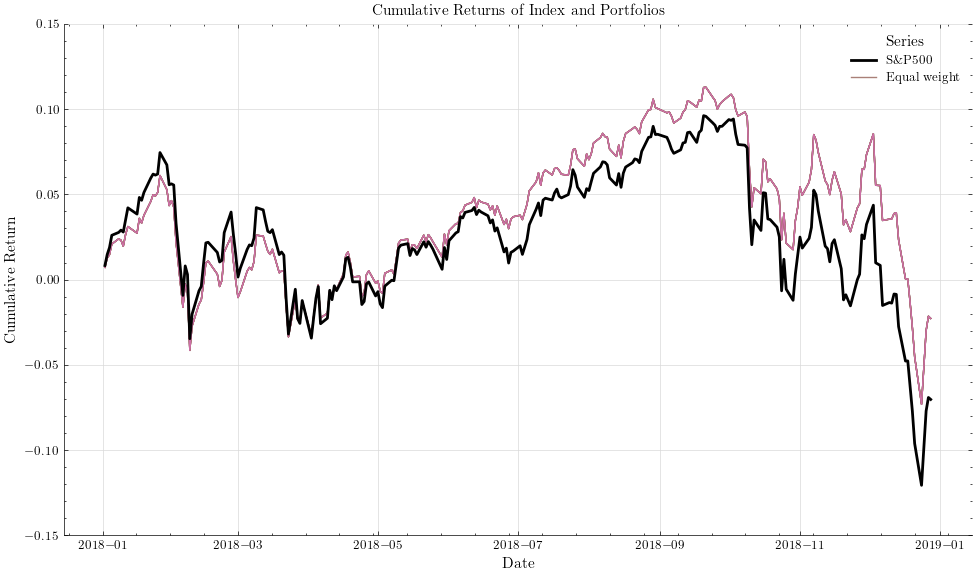
\includegraphics[width=\textwidth]{plots/results/equal_w_cum_ret_plot.png}
    \caption{Cumulative returns of S\&P500 and sector rotation strategies (2018)}\label{fig:eq_w_cum_ret_plot}
\end{figure}


\begin{table}[ht]
\centering
\caption{Descriptive Statistics of Index and Portfolio Returns}
\label{tab:return_stats_1}
\begin{tabular}{lrrrrrrr}
\toprule
{} & \multicolumn{1}{c}{Cumulative} & \multicolumn{1}{c}{Annualised} & \multicolumn{1}{c}{Annualised} & \multicolumn{1}{c}{Alpha} & \multicolumn{1}{c}{Information} & \multicolumn{1}{c}{PSR} & \multicolumn{1}{c}{PSR} \\
{} & \multicolumn{1}{c}{Return} & \multicolumn{1}{c}{Return} & \multicolumn{1}{c}{Volatility} & {} & \multicolumn{1}{c}{Ratio} & \multicolumn{1}{c}{(S*=0)} & \multicolumn{1}{c}{(S*=0.1)} \\
\midrule
S\&P500 & -7.03\% & -7.08\% & 17.06\% & 0.00\% & -- & -- & -- \\
equal\_weight & -2.27\% & -2.29\% & 15.39\% & 4.79\% & 0.29 & 0.92 & 0.45 \\
\bottomrule
\end{tabular}
\end{table}


To gauge risk-adjusted performance of the strategy, we report each portfolio's cumulative return, its active return relative to the S\&P500 (or 'Alpha'), and two spread sensitive statistics: the Information Ratio (IR) and the probabilistic Sharpe Ratio (PSR) at benchmark Sharpe thresholds $S^{*}=0$ and $S^{*}=0.1$. The IR evaluates excess return per unit of tracking-error volatility,

\begin{equation}
\mathrm{IR}=\frac{\mathbb{E}\left[R_{p}-R_{b}\right]}{\sigma\left(R_{p}-R_{b}\right)},
\end{equation}

where $R_{p}$ and $R_{b}$ are portfolio and benchmark returns, respectively, and a higher value signals more efficient investment relative to the risk taken by the investor. For example, an IR of below 0.1 means the strategy generates less than 0.1 units of excess return per unit of tracking error volatility, signaling that its returns are too small relative to their risk to justify strategy implementation. The PSR estimates the posterior probability that the true Sharpe ratio of a strategy exceeds a user-defined benchmark $S^{*}$,

\begin{equation}
\mathrm{PSR}= \Phi\left[\frac{\left(\hat{S}-S^{*}\right)\sqrt{T-1}}{\sqrt{1-\hat{S}^{2}/2}}\right],
\end{equation}
with $\hat{S}$ the sample Sharpe, $T$ the number of observations, and $\Phi(\cdot)$ the standard-normal cdf. Following \citeA{simonian_2019}, we report the PSR at $S^{*}=0$ and $S^{*}=0.1$.


The cumulative return chart for the in \cref{fig:cum_ret_plot} together with the summary statistics in \cref{tab:unconstr} shows the effectiveness of the active unconstrained sector rotation strategies relative to a passive S\&P 500 benchmark buy and hold strategy. While the index declined by 7.03\% over 2018\footnote{Due to ommitted data on 30/12/2018, 2018 period ends on 29/12/2018.}, 7 out of 8 models specifications outperformed the S\&P500 index, and 4 out of 8 specifications made positive returns despite the market conditions. The plot further shows that these active portfolios not only outperformed during the steady upswing through September but also sucessfully adjusted to the sudden sell off and increased volatility from mid-October onward, thereby dampening the loss.

A closer inspection reveals three surprises. First, the top three performers are all RF specifications, yet the fourth-best is an OLS specification. RF-C4f-EN is the best specification, achieving a cumulative return of 5.19\%, translating into an alpha of 12.31\%, an IR of 0.29 and a PSR of 0.97 at the 0.0 Sharpe benchmark.  Second, among RF variants the base FF5 variant outperforms its liquidity and sentiment enhanced variant. Opposite to that, the base RF C4F variant yield negative returns and performed worse than the enhanced OLS FF5 variant, while its enhanced c4f version is the best performing model. Third,  the only portfolio that underperformed the index was the base OLS FF5 (-10.66\%), while its enhanced specification is the only OLS model that generates a postive return, which confirms that both the additional liquidity and sentiment factors are crucial when momentum is missing. Another interesting observation is the RF enhanced models that are C4F variants yield better than their FF5 counterpart. This is probably due to momentum having a particularly strong effect in the macroeconomic environment of 2018, and profitability and investment factors delivered little incremental information.

The constrained strategy,which its statistics are reported in \cref{tab:constr} and \cref{fig:constr_cum_ret_plot}, shows a much more conservative approach to sector weight attribution. Evidently, \cref{fig:constr_cum_ret_plot} shows a much more tight clustering around the S\&P 500, while the unconstrained strategy fans out more. We could see in \cref{tab:constr} that, as expected,the order of the model performance stays exactly the same as the unconstrained model. An advantage of this strategy is that even for OLS models that underperformed against the S\&P500 in unconstrained strategy, the constrained strategy still outperformed the index. Even OLS base FF5 models, which had an active return of -3.58\%, had a positive return of 1.55\% in the constrained strategy. Similarly, OLS base c4f received a bump in active return of 2.2\%, comparing to the unconstrained strategy. What is surprising is that OLS enhanced C4F got lower active returns in the unconstrained strategy (3.2\%), compared to a 4.57\% increase in active returns in the constrained strategy.However, with lower risks comes lower returns. With the top 4 models, the unconstrained strategy got anywhere from 3 to 5\% more active returns than the constrained strategy.

However, implementing these models in actual trading applications requires much more than looking at raw return percentages. Each winning specification shows an IR of only 0.2-0.3, meaning that for every unit of active risk the strategy earns merely 0.2 to 0.3 units of excess return. This level of IR is considered modest at best, since institutional managers typically seek IRs above 0.5 to justify the costs and capacity constraints of active rotation \cite{gratton_2025}. The probabilistic Sharpe ratio at $S^{*} = 0$  with values around 40-60\% implying low confidence that the true Sharpe is larger than zero. In practice, one would prefer PSRs above 90\% at the target Sharpe to ensure robustness against estimation error. It essentially tell investors how likely they will make a positive return relative to the risk taken. In this case, we cannot reject the hypothesis that the true Sharpe ratio is zero. This is understandable given the volatility profile of 2018, where it is extremely uncertain that there would be any positive returns for any strategy. When we refer to the descriptive statistics of 2018, we could see how risky the market is.  Further research, with more computational resources could extend these strategies on a longer horizon (for example, using hold out set of 2016-2018), to have a more accurate outlook on the performance of these underlying models in less volatile periods.



% - Incredible results. Looking at the fig we could see that almost all of  the active strategies are outperforming the buy and hold index strategy. First four models, in a year where Sp500 index loses 7.03%, our strategy were able to hedge against that and even made positive returns. Only one model out of 8 lost against the index
% - In the fig we see that even  the plunge from mid october and volatile times at the end of the year , our models adjusted to that extremely well and generate signals that could hedge against the liquidity risk and sentiment shift
% - Looking closer: top 3 models are rf specification, but extremely surprising that 4rth is ols. Looking deeper in the top 4, c4f enhanced performed best with the cummulative ret =5.19\%, achieving an active return of 12.31\% . surprising that c4f is on top not ff5 {WHY DO YOU THINK c4f is on top not ff5}. even more surprising is that rf_base ff5 seems to beat rf_enhanced_ff5. {WHY IS THIS THE CASE}, with 11.44 active return comapred to 10.65\% active return. Most surpirasing of all, however, is that the 4rth place is not rf but an ols model, specifically ols_en_ff5 {WHY IS THIS POSSIBLE?}

% - Bottom 4 models: rf_base_c4f lost money {WHY enhanced do so good but base lost?}. Contrary to the hypothesis, ols base models performed worse than the ols enhanced, specifically c4f >ff5. Ols_base ff5 is the only one that lost money {WHY?}



\begin{figure}[H]
    \centering
    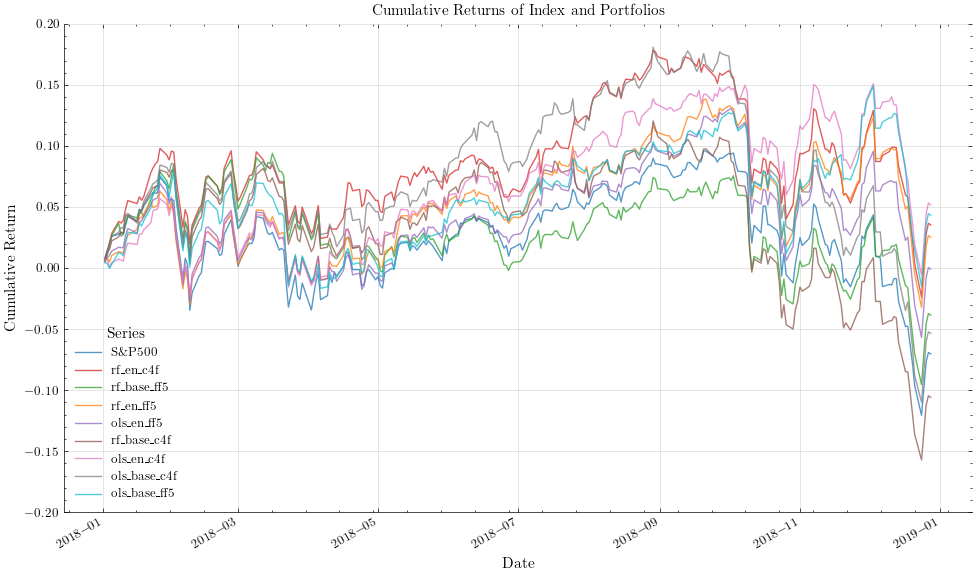
\includegraphics[width=\textwidth]{plots/results/cum_ret_plot.png}
    \caption{Cumulative returns of S\&P500 and sector rotation strategies (2018)}\label{fig:cum_ret_plot}
\end{figure}



% \begin{table}[ht]
% \centering
% \caption{Descriptive Statistics of Index and Portfolio Returns}
% \label{tab:unconstr}
% \begin{tabular}{lrrrrrrr}
% \toprule
% {} & \multicolumn{1}{c}{Cumulative} & \multicolumn{1}{c}{Annualised} & \multicolumn{1}{c}{Annualised} & \multicolumn{1}{c}{Alpha} & \multicolumn{1}{c}{Information} & \multicolumn{1}{c}{PSR} & \multicolumn{1}{c}{PSR} \\
% {} & \multicolumn{1}{c}{Return} & \multicolumn{1}{c}{Return} & \multicolumn{1}{c}{Volatility} & {} & \multicolumn{1}{c}{Ratio} & \multicolumn{1}{c}{(S*=0)} & \multicolumn{1}{c}{(S*=0.1)} \\
% \midrule
% S\&P500 & -7.03\% & -7.08\% & 17.06\% & 0.00\% & -- & -- & -- \\
% rf\_en\_c4f & 5.19\% & 5.23\% & 15.72\% & 12.31\% & 0.29 & 0.97 & 0.61 \\
% rf\_base\_ff5 & 4.33\% & 4.36\% & 16.45\% & 11.44\% & 0.28 & 0.95 & 0.57 \\
% rf\_en\_ff5 & 3.54\% & 3.57\% & 16.55\% & 10.65\% & 0.29 & 0.95 & 0.55 \\
% ols\_en\_ff5 & 2.53\% & 2.55\% & 16.27\% & 9.63\% & 0.28 & 0.95 & 0.53 \\
% rf\_base\_c4f & -0.08\% & -0.08\% & 16.10\% & 7.00\% & 0.26 & 0.93 & 0.48 \\
% ols\_en\_c4f & -3.85\% & -3.89\% & 16.48\% & 3.20\% & 0.22 & 0.89 & 0.38 \\
% ols\_base\_c4f & -5.34\% & -5.38\% & 17.23\% & 1.70\% & 0.21 & 0.86 & 0.33 \\
% ols\_base\_ff5 & -10.58\% & -10.66\% & 17.14\% & -3.58\% & 0.15 & 0.78 & 0.22 \\
% \bottomrule
% \end{tabular}
% \end{table}


% \begin{table}[ht]
% \centering
% \caption{Descriptive Statistics of Index and Portfolio Returns}
% \label{tab:constr}
% \begin{tabular}{lrrrrrrr}
% \toprule
% {} & \multicolumn{1}{c}{Cumulative} & \multicolumn{1}{c}{Annualised} & \multicolumn{1}{c}{Annualised} & \multicolumn{1}{c}{Alpha} & \multicolumn{1}{c}{Information} & \multicolumn{1}{c}{PSR} & \multicolumn{1}{c}{PSR} \\
% {} & \multicolumn{1}{c}{Return} & \multicolumn{1}{c}{Return} & \multicolumn{1}{c}{Volatility} & {} & \multicolumn{1}{c}{Ratio} & \multicolumn{1}{c}{(S*=0)} & \multicolumn{1}{c}{(S*=0.1)} \\
% \midrule
% S\&P500 & -7.03\% & -7.08\% & 17.06\% & 0.00\% & -- & -- & -- \\
% rf\_en\_c4f & -0.05\% & -0.05\% & 15.22\% & 7.03\% & 0.30 & 0.94 & 0.51 \\
% rf\_base\_ff5 & -0.29\% & -0.29\% & 15.39\% & 6.79\% & 0.30 & 0.93 & 0.50 \\
% rf\_en\_ff5 & -0.52\% & -0.53\% & 15.48\% & 6.55\% & 0.31 & 0.93 & 0.49 \\
% ols\_en\_ff5 & -0.83\% & -0.83\% & 15.45\% & 6.25\% & 0.30 & 0.93 & 0.48 \\
% rf\_base\_c4f & -1.59\% & -1.61\% & 15.42\% & 5.47\% & 0.29 & 0.92 & 0.46 \\
% ols\_en\_c4f & -2.71\% & -2.73\% & 15.43\% & 4.35\% & 0.27 & 0.91 & 0.43 \\
% ols\_base\_c4f & -3.16\% & -3.18\% & 15.66\% & 3.90\% & 0.27 & 0.91 & 0.42 \\
% ols\_base\_ff5 & -4.80\% & -4.84\% & 15.65\% & 2.24\% & 0.23 & 0.89 & 0.37 \\
% \bottomrule
% \end{tabular}
% \end{table}

%NEWWWWWWWWWWWWWWWW
\begin{table}[H]
\centering
\caption{Index and Portfolio Returns: Unconstrained Strategy}
\label{tab:unconstr}
\begin{tabular}{lrrrrrrr}
\toprule
{} & \multicolumn{1}{c}{Cumulative} & \multicolumn{1}{c}{Annualised} & \multicolumn{1}{c}{Annualised} & \multicolumn{1}{c}{Alpha} & \multicolumn{1}{c}{Information} & \multicolumn{1}{c}{PSR} & \multicolumn{1}{c}{PSR} \\
{} & \multicolumn{1}{c}{Return} & \multicolumn{1}{c}{Return} & \multicolumn{1}{c}{Volatility} & {} & \multicolumn{1}{c}{Ratio} & \multicolumn{1}{c}{(S*=0)} & \multicolumn{1}{c}{(S*=0.1)} \\
\midrule
S\&P500 & -7.03\% & -7.08\% & 17.06\% & 0.00\% & -- & -- & -- \\
rf\_en\_c4f & 5.19\% & 5.23\% & 15.72\% & 12.31\% & 0.29 & 0.61 & 0.10 \\
rf\_base\_ff5 & 4.33\% & 4.36\% & 16.45\% & 11.44\% & 0.28 & 0.59 & 0.09 \\
rf\_en\_ff5 & 3.54\% & 3.57\% & 16.55\% & 10.65\% & 0.29 & 0.57 & 0.08 \\
ols\_en\_ff5 & 2.53\% & 2.55\% & 16.27\% & 9.63\% & 0.28 & 0.55 & 0.07 \\
rf\_base\_c4f & -0.08\% & -0.08\% & 16.10\% & 7.00\% & 0.26 & 0.49 & 0.05 \\
ols\_en\_c4f & -3.85\% & -3.89\% & 16.48\% & 3.20\% & 0.22 & 0.40 & 0.03 \\
ols\_base\_c4f & -5.34\% & -5.38\% & 17.23\% & 1.70\% & 0.21 & 0.37 & 0.03 \\
ols\_base\_ff5 & -10.58\% & -10.66\% & 17.14\% & -3.58\% & 0.15 & 0.25 & 0.01 \\
\bottomrule
\end{tabular}
\end{table}

\begin{figure}[H]
    \centering
    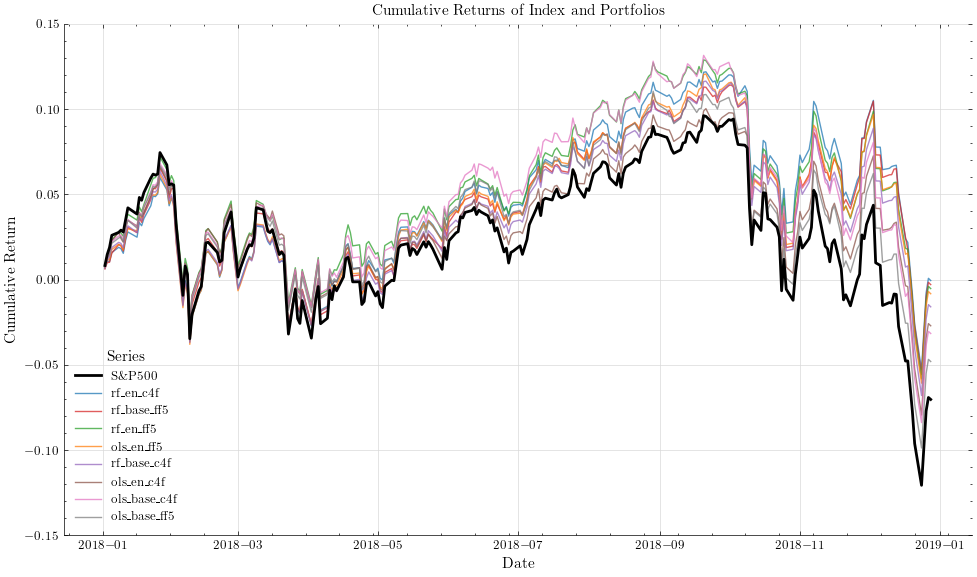
\includegraphics[width=\textwidth]{plots/results/contrained_cum_ret_plot.png}
    \caption{Cumulative returns of S\&P500 and sector rotation strategies (2018)}\label{fig:constr_cum_ret_plot}
\end{figure}

\begin{table}[H]
\centering
\caption{Index and Portfolio Returns: Constrained Strategy}
\label{tab:constr}
\begin{tabular}{lrrrrrrr}
\toprule
{} & \multicolumn{1}{c}{Cumulative} & \multicolumn{1}{c}{Annualised} & \multicolumn{1}{c}{Annualised} & \multicolumn{1}{c}{Alpha} & \multicolumn{1}{c}{Information} & \multicolumn{1}{c}{PSR} & \multicolumn{1}{c}{PSR} \\
{} & \multicolumn{1}{c}{Return} & \multicolumn{1}{c}{Return} & \multicolumn{1}{c}{Volatility} & {} & \multicolumn{1}{c}{Ratio} & \multicolumn{1}{c}{(S*=0)} & \multicolumn{1}{c}{(S*=0.1)} \\
\midrule
S\&P500 & -7.03\% & -7.08\% & 17.06\% & 0.00\% & -- & -- & -- \\
rf\_en\_c4f & -0.05\% & -0.05\% & 15.22\% & 7.03\% & 0.30 & 0.48 & 0.05 \\
rf\_base\_ff5 & -0.29\% & -0.29\% & 15.39\% & 6.79\% & 0.30 & 0.48 & 0.05 \\
rf\_en\_ff5 & -0.52\% & -0.53\% & 15.48\% & 6.55\% & 0.31 & 0.47 & 0.05 \\
ols\_en\_ff5 & -0.83\% & -0.83\% & 15.45\% & 6.25\% & 0.30 & 0.46 & 0.05 \\
rf\_base\_c4f & -1.59\% & -1.61\% & 15.42\% & 5.47\% & 0.29 & 0.44 & 0.04 \\
ols\_en\_c4f & -2.71\% & -2.73\% & 15.43\% & 4.35\% & 0.27 & 0.41 & 0.04 \\
ols\_base\_c4f & -3.16\% & -3.18\% & 15.66\% & 3.90\% & 0.27 & 0.40 & 0.03 \\
ols\_base\_ff5 & -4.80\% & -4.84\% & 15.65\% & 2.24\% & 0.23 & 0.36 & 0.03 \\
\bottomrule
\end{tabular}
\end{table}

\subsection{Discussion}
\subsubsection{Research Questions}

% \begin{enumerate}
%     \item \textbf{Research question 1}\
%     \textit{Does augmenting established linear asset-pricing models with liquidity-risk and sentiment factors, estimated via Random Forests, yield significantly higher out-of-sample explanatory power while retaining interpretability?}
%     \item \textbf{Research question 2}\
%     \textit{Given such an RF-based enhanced factor model, can its forecasts be combined with association-rule learning to derive simple, transparent sector-rotation rules that outperform the S\&P 500 index?}
%     \end{enumerate}

% Research question 1: Does augmenting established linear asset-pricing models with liquidity-risk and sentiment factors, estimated via Random Forests, yield significantly higher out-of-sample explanatory power while retaining interpretability?
% - Including liquidity risk and sentiment factors with Random Forest do yield a significantly higher out-of-sample explanatory power, compare to the baseline linear OLS models. However, it did not yield significantly higher out-of-sample explanatory power, compare to the baseline RF models.
% - Interpretaility approaches , though robust, is not as useful and strong as OLS's approach for financial practitioners. Method suggested by \citeA{simonian_2019}, in this analysis, produces uncamparable results to OLS counter parts, less informative, and lack statistical significance. How ever we could still get there with various alternatives (feature importance, shap, permutation importance) to see effect of each Fama french, liquidity, and sentiment factors on excess returns.
The findings of this thesis partly support the first research question. Enhancing the baseline C4F and  FF5 specifications with liquidity proxies (e.g.\ bid-ask spread, turnover, $ILLQ$) and the time varying sentiment index of \citeA{ung_2024} increases the out-of-sample $R^{2}$ and reduces hold out set forecast errors relative to plain-vanilla OLS benchmarks.  The gains, however, disappear once we benchmark RF against its own variants. It appears the tree ensemble already captures the same non-linearities and that liquidity and sentiment does not seem to significantly add forecasting power to the nonparametric model. In terms of interpretability, global coefficients from OLS remain easier for financial practitioners and managers to digest than feature importances from RF. The pseudo-beta approach proposed by \citeA{simonian_2019} is not only unsuitable for this particular empirical research, it also lacks the statisitcal rigour to be considered a valid substitute. However, when the primary objective is accurate forecasting, model-agnostic interpretability techniques (such as feature importance measures, SHAP values, and partial dependence plots) can elucidate the key drivers of returns in non-parametric models.


% Research Question 2: Given such an RF-based factor model, can its forecasts be combined with association-rule learning to derive simple, transparent sector-rotation rules that outperform the S\&P 500 index?
% - Yes. In both constrained and unconstrained strateies, ARL using RF forecasted rule outperforms S\&P 500 index. Through an empirical test, though we cannot definitely say due to only one year of backtesting, the enhancement factors in random forest models will not harm the performance of the rule-based strategy. Including them is seems to always be better than not. No overfitting/underfitting problems in our dataset. One strong evidence is our enhanced RF models are among the top performing models in the sector rotation strategy. For non-parametric models and for trading purposes, it seems like C4F and FF5 choice entirely depends on macroeconomic factors. 

%todo: Diebold–Mariano maybe?

This paper's approach and its findings support the second research question. Both the unconstrained and turnover-constrained implementations beat the S\&P500 on total return during the 2018 out-of-sample window, with no signs of over- or under-fitting. The inclusion of liquidity and sentiment factors never degrades strategy performance and, in most cases, improves it. The enhanced variant consistently rank among the top performers in the sector rotation strategy. Finally, the relative merits of $C4F$ versus $FF5$ inputs appear to hinge on current macroeconomic conditions rather than on any inherent superiority of one factor set over the other.

In terms of explainability, the framework developed in this paper delivers both the predictive accuracy of non-parametric learners and the transparency afforded by model-agnostic interpretability methods and rule-based trading signals. On any trading day, an individual forecast can be decomposed into the ARL sector rotation rule that generated the signal. That rule itself can be further can be traced back to each allocation decision back to specific Fama-French, liquidity, and sentiment factors via FI rankings (e.g.\ permutation importance or SHAP values), ensuring that every component of the prediction pipeline remains auditable and economically interpretable.

Nevertheless, the evidence should be regarded as preliminary and purely empirical: (i) only a single-year walk-forward evaluation of the expanding-window scheme has been completed, whereas a 20-year rolling back-test is required for robust inference; and (ii) the manual ARL support/confidence thresholds can make the rule set unstable. Replacing ARL with \emph{RuleFit}—a sparse additive rule ensemble—would fuse forecasting and explainability in one algorithm, avoid arbitrary thresholds, and yield naturally interpretable sector signals.

\subsubsection{Limitations}
% - Though we implemented extending window, computing resources limitataitons does not allow me to do 2 decades backtest. Ideally, this analysis should be doen with a proper extending window: train for X numbers of days lookback-> test day after. Then extend window. THen repeat for 20 years. THis paper did do the extending window continous retraining with extending window frame of 1 training year for 20 years. However it is reported as out-of-bag score only. With only 1 year to test out the extending window, it is not ideal. However it got a proxy what the actual result would be.

% - Constraints of ARL: This rule based method is based on manual threshold. Something of recent research, like RuleFit would be better. We are doing RF+ARL -> signals. However Rulefit does not need to be combined with anything else. It could create rules directly as a feature of the algo. These re actual if-then rules, such as "if market return >alpha and turn<= beta and news_sent> gamma then excess_return = 10\%".

% - Cannot statisically proof that either C4F or FF5 is better. But does not seem to entirely matter to non parametric models as we could include both (for forecasting purposes) SHAP, PDP and Feature Importance are only informative, not statisical proofs.
Despite implementing an expanding-window scheme, our back-test remains confined to a single year of walk-forward evaluation due to computational constraints. Ideally, we would train on an initial lookback of $X$ trading days, test on the subsequent day, then extend the training window and repeat this process continuously over a 20-year period. While this paper reports out of bag performance for a one-year training frame across two decades, the absence of a full dataset rolling back test in our study limits the robustness of our conclusions. Our one year proxy, however, suggests that the expanding window approach would likely produce comparable results over a longer time frame.

The ARL relies on manually selected support and confidence thresholds, which may render the extracted “if-then” sector-rotation rules sensitive to arbitrary parameter choices. Recent advances—such as the \texttt{RuleFit} algorithm, which generate sparse, additive rule ensembles directly from the data without the need for external rule mining and threshold tuning. By integrating rule extraction into the learner itself, RuleFit produces concise, interpretable rules (e.g.\ \emph{if} market return $>$ $\alpha$ \emph{and} turnover $\le \beta$ \emph{and} sentiment $>$ $\gamma$, \emph{then} excess return $=10\%$) while avoiding the two-step RF+ARL pipeline.

Finally, we cannot statistically demonstrate that the C4F or FF5 formulations are superior within a non-parametric forecasting framework. In practice, RF models can accommodate both factor sets simultaneously and simply don't split on redudant predictors. Moreover, interpretability tools—feature importance, SHAP values, and PDP—offer descriptive insights into factor contributions but do not constitute formal hypothesis tests. Future work should incorporate inferential procedures (e.g.\ testing differences in out-of-sample $R^2$ or using bootstrap confidence intervals for SHAP contributions) to underpin the economic relevance of each factor choice.

\subsubsection{How investors and asset managers can use the findings of this paper}
% - ideal workflow: gather past data -> plug in -> auto feature engineers_> pipeline (rf -> arl-> rules) -> weighting on tomorrows sector. Tomorrow comes, automatcially include today in traning window, adjust for todays excess returns -> forecast tomorrow -> weight tomorrow..
% - When an actual trade is not as expected -> can go back and see exactly which factor caused the trade to be not as expected with feature importance, shap, pdp
% - With incorporation of sentiment, liquidity risks, can think about other macroeconomic factoers that are less niche, since the two most promonient factors are taken into account. Help financial professional make better decisions that are always explainable at every single step of the trading route
For asset managers, this is the proposed pipeline: automated data ingestion $\rightarrow$ feature engineering $\rightarrow$ RF forecasting $\rightarrow$ rule extraction. This pipeline delivers a daily sector-weight vector whose rationale can be traced factor-by-factor. When live trades deviate from expectations, global and local attribution via feature importance, SHAP, or partial dependence immediately isolates which of the traditional FF factors ($SMB$, $HML$, $MOM$, $RMW$, $CMA$), the liquidity variables, or the sentiment index drove the surprise deviation. Because liquidity risk and sentiment already proxy two of the most pervasive macro drivers, practitioners can next experiment with complementary state variables (e.g.\ term-structure slope, credit spreads) without materially inflating model complexity.


% \noindent\textbf{Recommended refinements and theoretical checks}
% \begin{itemize}
% \item \emph{Statistical testing}: report out-of-sample $\Delta R^{2}$ p-values and Diebold-Mariano statistics to demonstrate that RF-based enhancements are materially better than OLS and not materially worse than vanilla RF.
% \item \emph{Factor choice}: clarify why $C4F$ vs.\ $FF5$ matters once non-parametric learners are used; consider including both sets of factors and letting the algorithm down-weight redundant ones.
% \item \emph{Back-test design}: extend the expanding-window evaluation to the full 1990-2018 span; document walk-forward hyper-parameter tuning to avoid look-ahead bias.
% \item \emph{Interpretability caveat}: remind readers that SHAP and permutation scores are \emph{not} formal statistical betas; they measure marginal predictive contribution, not economic elasticity.
% \item \emph{Liquidity–sentiment theory}: verify that liquidity betas indeed earn a premium during market stress (e.g.\ 2008, 2020) and that sentiment loads interact with the size factor, as implied by \citeA{baker_wurgler_2007}.
% \end{itemize}
\section{Conclusion} \label{sec:conclusion}
	
In conclusion, our findings show that augmenting the traditional C4F and FF5 frameworks with liquidity and investor sentiment information yields targeted but meaningful out-of-sample gains while preserving the transparency that makes non-parametric models attractive to practitioners. Shifting from OLS to RF already multiplies explanatory power around six fold and cuts hold-out errors by roughly 100\%, validating the use of tree ensembles for sector level return forecasting. Layering in the liquidity proxies and the sentiment index produces a second, more nuanced improvement. Forecast accuracy rises significantly (at the 95 \% confidence level or better) in those sectors where illiquidity shocks or behavioural swings matter most (Energy, Materials, Industrials, Utilities and Real Estate in the C4F setting, and all but two sectors in the FF5 setting). Crucially, the models' interpretability is not sacrificed, the pseudo-betas retain the familiar economic meaning of linear betas, allowing finance professionals to trace why predictions move when either traditional or alternative factors change. In sum, enhancing multifactor asset-pricing models with carefully chosen liquidity and sentiment signals delivers sector-specific predictive benefits on top of the sizeable RF baseline gains, all while keeping the rule-based intuition and pseudo-beta diagnostics that render the non-parametric approach practically usable.

We translate each model's predicted excess returns into a straightforward daily rule sets that generates signals for the trading models to automatically assign weights between sectors. Using this approach, signals from liquidity risk and sentiment enhanced Random Forest and OLS models outperform the benchmark S\&P 500 in the volatile 2018 period.  Seven of eight unconstrained strategies beat the index and four generated positive absolute returns, with the RF-C4F-E as the best sector rotation strategy model, which shows +5.19\% alpha. However, the Sharpe ratio cannot be statistically proven to be larger than 0, meaning that the returns on investments does not outweigh the risk taken. Therefore, we cannot concretely conclude that the models produce trading signals that will statisically be outperforming the S\&P500. Nevertheless, the results are very promising. Both the models' gains compared to the benchmark index are present in both constrained and unconstrained strategies. The nature of the 2018 dataset could be a part of the reason that the risks outweighs the returns of the models. With more computation, it would be more statisically sound if the same back-test were to be applied for the whole dataset so that we could have a wider range of results to draw conclusions from.


\newpage
\bibliographystyle{apacite} 
\bibliography{ref_masterthesis} 

\newpage
\appendix
\section{Appendix} \label{sec:appendix}
\subsection{Github repository}
You can find the Git Repo here

The visual plots are designed using \citeA{scienceplots}.

The formatting of tables and figures are APA.

Models trained using statsmodels, sklearn, imodels.

Used pandas for data manipulation.

\begin{table}[ht]
    \centering

    
    \caption{Descriptive Statistics for Sector: 20 (1/2)}
    \label{tab:sec20_a}
    
    \begin{tabular}{lcccccc}
    \toprule
    Statistic & $prc$ & $ret$ & $excess_ret$ & $vol$ & $baspread$ & $put_call_ratio$ \\\midrule
    N & 5282 & 5282 & 5282 & 5282 & 5282 & 5282 \\
    Mean & 70.168 & 0.001 & 0.000 & 9828999.019 & 1.469 & 1.475 \\
    SD & 28.023 & 0.013 & 0.013 & 6934471.039 & 0.793 & 1.764 \\
    Min & 29.269 & -0.087 & -0.087 & 831257.778 & 0.396 & 0.309 \\
    Q1 & 50.274 & -0.006 & -0.006 & 6144046.127 & 0.987 & 0.926 \\
    Median & 61.637 & 0.001 & 0.001 & 8235043.176 & 1.277 & 1.176 \\
    Q3 & 85.891 & 0.007 & 0.007 & 11555892.003 & 1.683 & 1.582 \\
    Max & 167.178 & 0.101 & 0.101 & 112980490.977 & 10.786 & 81.939 \\
    \bottomrule
    \end{tabular}

    \end{table}
    
    \begin{table}[ht]
    \centering

    
    \caption{Descriptive Statistics for Sector: 20 (2/2)}
    \label{tab:sec20_b}
    
    \begin{tabular}{lcccc}
    \toprule
    Statistic & $turn$ & $mvel1$ & $dolvol$ & $daily_illq$ \\\midrule
    N & 5282 & 5282 & 5282 & 5282 \\
    Mean & 5.838 & 18.354 & 628767649.146 & 0.000 \\
    SD & 2.646 & 0.443 & 384717986.617 & 0.000 \\
    Min & 0.897 & 16.905 & 58406854.478 & 0.000 \\
    Q1 & 3.932 & 18.087 & 389901206.851 & 0.000 \\
    Median & 5.400 & 18.255 & 567946979.622 & 0.000 \\
    Q3 & 7.077 & 18.641 & 766602866.312 & 0.000 \\
    Max & 25.564 & 19.557 & 6430725101.514 & 0.000 \\
    \bottomrule
    \end{tabular}

    \end{table}
    
    \begin{table}[ht]
    \centering

    
    \caption{Descriptive Statistics for Sector: 30 (1/2)}
    \label{tab:sec30_a}
    
    \begin{tabular}{lcccccc}
    \toprule
    Statistic & $prc$ & $ret$ & $excess_ret$ & $vol$ & $baspread$ & $put_call_ratio$ \\\midrule
    N & 5282 & 5282 & 5282 & 5282 & 5282 & 5282 \\
    Mean & 59.499 & 0.000 & 0.000 & 6271026.555 & 1.084 & 1.287 \\
    SD & 12.371 & 0.010 & 0.010 & 2872717.134 & 0.497 & 1.936 \\
    Min & 37.737 & -0.070 & -0.070 & 763120.878 & 0.371 & 0.274 \\
    Q1 & 49.980 & -0.004 & -0.004 & 4424177.211 & 0.757 & 0.847 \\
    Median & 55.264 & 0.001 & 0.001 & 5750033.075 & 0.953 & 1.051 \\
    Q3 & 66.692 & 0.005 & 0.005 & 7447012.648 & 1.276 & 1.334 \\
    Max & 93.151 & 0.095 & 0.095 & 30853127.738 & 9.232 & 83.144 \\
    \bottomrule
    \end{tabular}

    \end{table}
    
    \begin{table}[ht]
    \centering

    
    \caption{Descriptive Statistics for Sector: 30 (2/2)}
    \label{tab:sec30_b}
    
    \begin{tabular}{lcccc}
    \toprule
    Statistic & $turn$ & $mvel1$ & $dolvol$ & $daily_illq$ \\\midrule
    N & 5282 & 5282 & 5282 & 5282 \\
    Mean & 4.438 & 18.457 & 369821669.912 & 0.000 \\
    SD & 1.792 & 0.128 & 169482438.827 & 0.000 \\
    Min & 0.702 & 18.026 & 48896317.651 & 0.000 \\
    Q1 & 3.085 & 18.370 & 231200020.438 & 0.000 \\
    Median & 4.215 & 18.454 & 365031876.073 & 0.000 \\
    Q3 & 5.391 & 18.559 & 462721667.269 & 0.000 \\
    Max & 18.920 & 18.788 & 1608316986.315 & 0.000 \\
    \bottomrule
    \end{tabular}

    \end{table}
    
    \begin{table}[ht]
    \centering

    
    \caption{Descriptive Statistics for Sector: 50 (1/2)}
    \label{tab:sec50_a}
    
    \begin{tabular}{lcccccc}
    \toprule
    Statistic & $prc$ & $ret$ & $excess_ret$ & $vol$ & $baspread$ & $put_call_ratio$ \\\midrule
    N & 5282 & 5282 & 5282 & 5282 & 5282 & 5282 \\
    Mean & 136.093 & 0.001 & 0.000 & 11068977.133 & 2.750 & 1.424 \\
    SD & 108.892 & 0.013 & 0.013 & 5649685.083 & 2.486 & 3.634 \\
    Min & 25.002 & -0.086 & -0.086 & 1127806.462 & 0.313 & 0.151 \\
    Q1 & 42.823 & -0.006 & -0.006 & 7071211.218 & 1.270 & 0.722 \\
    Median & 100.603 & 0.001 & 0.001 & 10125347.386 & 2.098 & 0.942 \\
    Q3 & 189.016 & 0.007 & 0.007 & 13821541.101 & 3.375 & 1.325 \\
    Max & 492.768 & 0.143 & 0.143 & 80321872.659 & 34.141 & 181.739 \\
    \bottomrule
    \end{tabular}

    \end{table}
    
    \begin{table}[ht]
    \centering

    
    \caption{Descriptive Statistics for Sector: 50 (2/2)}
    \label{tab:sec50_b}
    
    \begin{tabular}{lcccc}
    \toprule
    Statistic & $turn$ & $mvel1$ & $dolvol$ & $daily_illq$ \\\midrule
    N & 5282 & 5282 & 5282 & 5282 \\
    Mean & 6.939 & 18.416 & 1695637364.583 & 0.000 \\
    SD & 3.116 & 0.476 & 1721244267.447 & 0.000 \\
    Min & 0.884 & 17.591 & 55595345.536 & 0.000 \\
    Q1 & 4.546 & 18.033 & 288494221.216 & 0.000 \\
    Median & 6.449 & 18.387 & 1496639053.806 & 0.000 \\
    Q3 & 8.708 & 18.755 & 2411439974.076 & 0.000 \\
    Max & 32.839 & 19.521 & 29753312709.727 & 0.000 \\
    \bottomrule
    \end{tabular}

    \end{table}
    
    \begin{table}[ht]
    \centering

    
    \caption{Descriptive Statistics for Sector: 40 (1/2)}
    \label{tab:sec40_a}
    
    \begin{tabular}{lcccccc}
    \toprule
    Statistic & $prc$ & $ret$ & $excess_ret$ & $vol$ & $baspread$ & $put_call_ratio$ \\\midrule
    N & 5282 & 5282 & 5282 & 5282 & 5282 & 5282 \\
    Mean & 64.786 & 0.001 & 0.001 & 16889210.353 & 1.488 & 1.528 \\
    SD & 18.267 & 0.019 & 0.019 & 21496826.183 & 0.783 & 1.527 \\
    Min & 25.285 & -0.163 & -0.163 & 684250.677 & 0.372 & 0.212 \\
    Q1 & 51.519 & -0.007 & -0.007 & 4758200.154 & 0.969 & 0.981 \\
    Median & 60.332 & 0.000 & 0.000 & 9322123.268 & 1.269 & 1.267 \\
    Q3 & 76.408 & 0.008 & 0.008 & 18289047.539 & 1.797 & 1.700 \\
    Max & 119.449 & 0.189 & 0.189 & 230471985.248 & 9.549 & 66.030 \\
    \bottomrule
    \end{tabular}

    \end{table}
    
    \begin{table}[ht]
    \centering

    
    \caption{Descriptive Statistics for Sector: 40 (2/2)}
    \label{tab:sec40_b}
    
    \begin{tabular}{lcccc}
    \toprule
    Statistic & $turn$ & $mvel1$ & $dolvol$ & $daily_illq$ \\\midrule
    N & 5282 & 5282 & 5282 & 5282 \\
    Mean & 7.027 & 18.189 & 972019713.412 & 0.000 \\
    SD & 5.794 & 0.340 & 997673071.368 & 0.000 \\
    Min & 0.785 & 16.796 & 43645914.858 & 0.000 \\
    Q1 & 3.807 & 18.001 & 253143365.899 & 0.000 \\
    Median & 4.966 & 18.226 & 741418271.883 & 0.000 \\
    Q3 & 7.857 & 18.399 & 1291657398.499 & 0.000 \\
    Max & 59.537 & 18.935 & 11605791822.857 & 0.000 \\
    \bottomrule
    \end{tabular}

    \end{table}
    
    \begin{table}[ht]
    \centering

    
    \caption{Descriptive Statistics for Sector: 15 (1/2)}
    \label{tab:sec15_a}
    
    \begin{tabular}{lcccccc}
    \toprule
    Statistic & $prc$ & $ret$ & $excess_ret$ & $vol$ & $baspread$ & $put_call_ratio$ \\\midrule
    N & 5282 & 5282 & 5282 & 5282 & 5282 & 5282 \\
    Mean & 63.011 & 0.001 & 0.001 & 3880837.508 & 1.483 & 2.068 \\
    SD & 23.070 & 0.015 & 0.015 & 2246579.968 & 0.679 & 3.554 \\
    Min & 29.172 & -0.115 & -0.115 & 255822.090 & 0.404 & 0.322 \\
    Q1 & 45.575 & -0.007 & -0.007 & 2170105.119 & 1.049 & 0.934 \\
    Median & 56.539 & 0.001 & 0.001 & 3438225.795 & 1.328 & 1.310 \\
    Q3 & 79.701 & 0.008 & 0.008 & 5102883.587 & 1.712 & 2.052 \\
    Max & 123.772 & 0.138 & 0.138 & 15549166.763 & 6.941 & 129.319 \\
    \bottomrule
    \end{tabular}

    \end{table}
    
    \begin{table}[ht]
    \centering

    
    \caption{Descriptive Statistics for Sector: 15 (2/2)}
    \label{tab:sec15_b}
    
    \begin{tabular}{lcccc}
    \toprule
    Statistic & $turn$ & $mvel1$ & $dolvol$ & $daily_illq$ \\\midrule
    N & 5282 & 5282 & 5282 & 5282 \\
    Mean & 8.914 & 17.030 & 254083019.109 & 0.000 \\
    SD & 5.041 & 0.324 & 167063658.330 & 0.000 \\
    Min & 0.874 & 16.476 & 12711807.515 & 0.000 \\
    Q1 & 5.382 & 16.783 & 90065337.750 & 0.000 \\
    Median & 7.454 & 16.965 & 259143499.663 & 0.000 \\
    Q3 & 11.035 & 17.209 & 371058212.164 & 0.000 \\
    Max & 39.742 & 18.027 & 1256358444.162 & 0.001 \\
    \bottomrule
    \end{tabular}

    \end{table}
    
    \begin{table}[ht]
    \centering

    
    \caption{Descriptive Statistics for Sector: 10 (1/2)}
    \label{tab:sec10_a}
    
    \begin{tabular}{lcccccc}
    \toprule
    Statistic & $prc$ & $ret$ & $excess_ret$ & $vol$ & $baspread$ & $put_call_ratio$ \\\midrule
    N & 5282 & 5282 & 5282 & 5282 & 5282 & 5282 \\
    Mean & 67.474 & 0.001 & 0.000 & 8546126.737 & 1.554 & 0.959 \\
    SD & 12.384 & 0.016 & 0.016 & 5046233.258 & 0.740 & 0.984 \\
    Min & 37.158 & -0.154 & -0.154 & 658309.207 & 0.385 & 0.128 \\
    Q1 & 59.928 & -0.008 & -0.008 & 5490141.126 & 1.099 & 0.658 \\
    Median & 68.434 & 0.001 & 0.001 & 7489574.039 & 1.401 & 0.837 \\
    Q3 & 76.515 & 0.009 & 0.009 & 10736086.038 & 1.805 & 1.068 \\
    Max & 96.369 & 0.186 & 0.186 & 58154106.223 & 9.172 & 38.256 \\
    \bottomrule
    \end{tabular}

    \end{table}
    
    \begin{table}[ht]
    \centering

    
    \caption{Descriptive Statistics for Sector: 10 (2/2)}
    \label{tab:sec10_b}
    
    \begin{tabular}{lcccc}
    \toprule
    Statistic & $turn$ & $mvel1$ & $dolvol$ & $daily_illq$ \\\midrule
    N & 5282 & 5282 & 5282 & 5282 \\
    Mean & 6.576 & 18.784 & 574719918.135 & 0.000 \\
    SD & 3.073 & 0.233 & 336137228.851 & 0.000 \\
    Min & 0.849 & 17.923 & 41783236.361 & 0.000 \\
    Q1 & 4.197 & 18.718 & 306691795.275 & 0.000 \\
    Median & 6.178 & 18.818 & 538633805.239 & 0.000 \\
    Q3 & 8.237 & 18.917 & 740427368.983 & 0.000 \\
    Max & 33.334 & 19.267 & 2968008042.642 & 0.000 \\
    \bottomrule
    \end{tabular}

    \end{table}
    
    \begin{table}[ht]
    \centering

    
    \caption{Descriptive Statistics for Sector: 45 (1/2)}
    \label{tab:sec45_a}
    
    \begin{tabular}{lcccccc}
    \toprule
    Statistic & $prc$ & $ret$ & $excess_ret$ & $vol$ & $baspread$ & $put_call_ratio$ \\\midrule
    N & 5282 & 5282 & 5282 & 5282 & 5282 & 5282 \\
    Mean & 75.478 & 0.001 & 0.001 & 24953036.918 & 1.870 & 0.899 \\
    SD & 44.235 & 0.018 & 0.018 & 10142132.829 & 1.321 & 0.484 \\
    Min & 25.415 & -0.094 & -0.094 & 2987333.033 & 0.349 & 0.213 \\
    Q1 & 36.373 & -0.007 & -0.007 & 17486775.078 & 0.925 & 0.681 \\
    Median & 69.912 & 0.001 & 0.001 & 24224608.717 & 1.465 & 0.825 \\
    Q3 & 98.228 & 0.009 & 0.009 & 31002896.990 & 2.405 & 1.010 \\
    Max & 246.234 & 0.178 & 0.178 & 107483726.264 & 13.527 & 19.662 \\
    \bottomrule
    \end{tabular}

    \end{table}
    
    \begin{table}[ht]
    \centering

    
    \caption{Descriptive Statistics for Sector: 45 (2/2)}
    \label{tab:sec45_b}
    
    \begin{tabular}{lcccc}
    \toprule
    Statistic & $turn$ & $mvel1$ & $dolvol$ & $daily_illq$ \\\midrule
    N & 5282 & 5282 & 5282 & 5282 \\
    Mean & 10.089 & 18.877 & 1673634455.577 & 0.000 \\
    SD & 3.370 & 0.443 & 912104160.507 & 0.000 \\
    Min & 1.765 & 18.020 & 195395936.138 & 0.000 \\
    Q1 & 7.638 & 18.530 & 1040191106.181 & 0.000 \\
    Median & 9.727 & 18.724 & 1401548247.960 & 0.000 \\
    Q3 & 11.978 & 19.242 & 2075148221.216 & 0.000 \\
    Max & 30.919 & 20.042 & 7751690972.753 & 0.000 \\
    \bottomrule
    \end{tabular}

    \end{table}
    
    \begin{table}[ht]
    \centering

    
    \caption{Descriptive Statistics for Sector: 55 (1/2)}
    \label{tab:sec55_a}
    
    \begin{tabular}{lcccccc}
    \toprule
    Statistic & $prc$ & $ret$ & $excess_ret$ & $vol$ & $baspread$ & $put_call_ratio$ \\\midrule
    N & 5282 & 5282 & 5282 & 5282 & 5282 & 5282 \\
    Mean & 47.957 & 0.000 & 0.000 & 2437339.653 & 0.907 & 1.909 \\
    SD & 11.675 & 0.012 & 0.012 & 1151191.169 & 0.478 & 2.611 \\
    Min & 28.470 & -0.087 & -0.087 & 208089.248 & 0.213 & 0.196 \\
    Q1 & 38.375 & -0.005 & -0.005 & 1579670.539 & 0.593 & 0.878 \\
    Median & 44.822 & 0.001 & 0.001 & 2395635.346 & 0.782 & 1.293 \\
    Q3 & 55.607 & 0.007 & 0.007 & 3115108.599 & 1.081 & 2.107 \\
    Max & 80.605 & 0.136 & 0.136 & 10617782.997 & 6.250 & 103.171 \\
    \bottomrule
    \end{tabular}

    \end{table}
    
    \begin{table}[ht]
    \centering

    
    \caption{Descriptive Statistics for Sector: 55 (2/2)}
    \label{tab:sec55_b}
    
    \begin{tabular}{lcccc}
    \toprule
    Statistic & $turn$ & $mvel1$ & $dolvol$ & $daily_illq$ \\\midrule
    N & 5282 & 5282 & 5282 & 5282 \\
    Mean & 5.728 & 16.731 & 119959829.125 & 0.000 \\
    SD & 2.181 & 0.373 & 67732465.355 & 0.000 \\
    Min & 0.788 & 15.981 & 8827933.518 & 0.000 \\
    Q1 & 4.258 & 16.446 & 65544177.449 & 0.000 \\
    Median & 5.507 & 16.731 & 113312619.099 & 0.000 \\
    Q3 & 6.855 & 16.989 & 160142759.928 & 0.000 \\
    Max & 20.315 & 17.463 & 565008316.911 & 0.001 \\
    \bottomrule
    \end{tabular}

    \end{table}
    
    \begin{table}[ht]
    \centering

    
    \caption{Descriptive Statistics for Sector: 35 (1/2)}
    \label{tab:sec35_a}
    
    \begin{tabular}{lcccccc}
    \toprule
    Statistic & $prc$ & $ret$ & $excess_ret$ & $vol$ & $baspread$ & $put_call_ratio$ \\\midrule
    N & 5282 & 5282 & 5282 & 5282 & 5282 & 5282 \\
    Mean & 71.063 & 0.001 & 0.001 & 7841459.146 & 1.567 & 1.134 \\
    SD & 30.558 & 0.012 & 0.012 & 3834773.771 & 0.860 & 0.990 \\
    Min & 34.810 & -0.088 & -0.089 & 727108.820 & 0.385 & 0.224 \\
    Q1 & 49.112 & -0.005 & -0.005 & 5304269.393 & 0.929 & 0.799 \\
    Median & 55.106 & 0.001 & 0.001 & 7114695.460 & 1.322 & 0.992 \\
    Q3 & 88.289 & 0.006 & 0.006 & 9727851.501 & 1.994 & 1.253 \\
    Max & 160.848 & 0.122 & 0.122 & 48011396.535 & 14.569 & 44.560 \\
    \bottomrule
    \end{tabular}

    \end{table}
    
    \begin{table}[ht]
    \centering

    
    \caption{Descriptive Statistics for Sector: 35 (2/2)}
    \label{tab:sec35_b}
    
    \begin{tabular}{lcccc}
    \toprule
    Statistic & $turn$ & $mvel1$ & $dolvol$ & $daily_illq$ \\\midrule
    N & 5282 & 5282 & 5282 & 5282 \\
    Mean & 5.648 & 18.297 & 511146534.102 & 0.000 \\
    SD & 2.069 & 0.219 & 240940546.520 & 0.000 \\
    Min & 0.892 & 17.678 & 64915884.729 & 0.000 \\
    Q1 & 4.251 & 18.128 & 326371265.004 & 0.000 \\
    Median & 5.356 & 18.299 & 488210791.596 & 0.000 \\
    Q3 & 6.733 & 18.490 & 643192757.551 & 0.000 \\
    Max & 19.620 & 18.790 & 2765935978.401 & 0.000 \\
    \bottomrule
    \end{tabular}

    \end{table}
    
    \begin{table}[ht]
    \centering

    
    \caption{Descriptive Statistics for Sector: 25 (1/2)}
    \label{tab:sec25_a}
    
    \begin{tabular}{lcccccc}
    \toprule
    Statistic & $prc$ & $ret$ & $excess_ret$ & $vol$ & $baspread$ & $put_call_ratio$ \\\midrule
    N & 5282 & 5282 & 5282 & 5282 & 5282 & 5282 \\
    Mean & 119.213 & 0.001 & 0.001 & 6914008.328 & 2.744 & 1.632 \\
    SD & 154.452 & 0.014 & 0.014 & 3182450.646 & 4.155 & 1.882 \\
    Min & 25.425 & -0.109 & -0.109 & 643261.398 & 0.462 & 0.382 \\
    Q1 & 40.354 & -0.006 & -0.006 & 4898102.104 & 1.034 & 1.003 \\
    Median & 51.929 & 0.001 & 0.001 & 6206102.108 & 1.579 & 1.259 \\
    Q3 & 128.601 & 0.008 & 0.008 & 8375971.556 & 2.673 & 1.709 \\
    Max & 903.422 & 0.120 & 0.120 & 35044429.055 & 62.182 & 54.589 \\
    \bottomrule
    \end{tabular}

    \end{table}
    
    \begin{table}[ht]
    \centering

    
    \caption{Descriptive Statistics for Sector: 25 (2/2)}
    \label{tab:sec25_b}
    
    \begin{tabular}{lcccc}
    \toprule
    Statistic & $turn$ & $mvel1$ & $dolvol$ & $daily_illq$ \\\midrule
    N & 5282 & 5282 & 5282 & 5282 \\
    Mean & 9.476 & 17.652 & 713993577.243 & 0.000 \\
    SD & 3.815 & 0.659 & 851459206.634 & 0.000 \\
    Min & 1.256 & 16.660 & 34524347.921 & 0.000 \\
    Q1 & 6.992 & 17.192 & 251254955.408 & 0.000 \\
    Median & 8.814 & 17.431 & 428488973.481 & 0.000 \\
    Q3 & 11.455 & 17.926 & 777369151.969 & 0.000 \\
    Max & 34.395 & 19.857 & 7490510908.258 & 0.001 \\
    \bottomrule
    \end{tabular}

    \end{table}
    
    \begin{table}[ht]
    \centering

    
    \caption{Descriptive Statistics for Sector: 60 (1/2)}
    \label{tab:sec60_a}
    
    \begin{tabular}{lcccccc}
    \toprule
    Statistic & $prc$ & $ret$ & $excess_ret$ & $vol$ & $baspread$ & $put_call_ratio$ \\\midrule
    N & 5282 & 5282 & 5282 & 5282 & 5282 & 5282 \\
    Mean & 70.656 & 0.001 & 0.001 & 1891716.017 & 1.600 & 3.585 \\
    SD & 26.333 & 0.019 & 0.019 & 1320184.227 & 0.889 & 14.631 \\
    Min & 25.941 & -0.164 & -0.164 & 123961.656 & 0.304 & 0.003 \\
    Q1 & 49.506 & -0.008 & -0.008 & 974650.222 & 1.020 & 0.924 \\
    Median & 63.544 & 0.001 & 0.001 & 1672814.565 & 1.408 & 1.680 \\
    Q3 & 85.261 & 0.008 & 0.008 & 2356931.009 & 1.944 & 3.019 \\
    Max & 129.417 & 0.199 & 0.199 & 10891439.527 & 13.545 & 641.121 \\
    \bottomrule
    \end{tabular}

    \end{table}
    
    \begin{table}[ht]
    \centering

    
    \caption{Descriptive Statistics for Sector: 60 (2/2)}
    \label{tab:sec60_b}
    
    \begin{tabular}{lcccc}
    \toprule
    Statistic & $turn$ & $mvel1$ & $dolvol$ & $daily_illq$ \\\midrule
    N & 5282 & 5282 & 5282 & 5282 \\
    Mean & 7.166 & 16.518 & 134819543.108 & 0.000 \\
    SD & 5.419 & 0.439 & 88899255.304 & 0.000 \\
    Min & 0.646 & 15.528 & 6012612.592 & 0.000 \\
    Q1 & 4.396 & 16.161 & 50523361.493 & 0.000 \\
    Median & 5.772 & 16.409 & 137837191.891 & 0.000 \\
    Q3 & 7.844 & 16.982 & 198296574.315 & 0.000 \\
    Max & 52.579 & 17.306 & 843176626.546 & 0.006 \\
    \bottomrule
    \end{tabular}

    \end{table}
    


\end{document}